% Commenti speciali

% !TEX encoding = UTF-8 Unicode
% !TEX TS-program = pdflatex
% !TEX spellcheck = it-IT
% !TEX root = Dispensa/af.tex

% Capitolo 2
\chapter{Equazioni ellittiche lineari del secondo ordine}\label{Equazioni ellittiche lineari del secondo ordine}
\section{Introduzione}
Nel seguito indicheremo con $\Delta = \sum_{j=1}^{n}\frac{\partial^2}{\partial x_j^2}$ l'operatore di Laplace, o Laplaciano. Altro non è che la traccia della matrice hessiana.

Iniziamo presentando l'esempio capostipite di tutta la teoria che intendiamo costruire.
\begin{esempio}\textbf{\emph{(problema di Poisson)}}\label{esempiopoisson}
	Siano $U$ limitato con $\partial U$ di classe $C^1$ ed $f \in L^2(U)$. Siamo interessati alle applicazioni $u$ che soddisfano 
	\begin{equation}\label{Poisson}
		\begin{cases}
			-\Delta u = f & \textup{in } U,\\
			u= 0 & \textup{su } \partial U.
		\end{cases}
	\end{equation}
	Se $f = 0$, chiamiamo tali applicazioni \emph{armoniche}.
	
	Data $f \in C(U)$, diciamo che $u$ è una \emph{soluzione classica del problema di Poisson} \eqref{Poisson}, se $u \in C^2(U)\cap C(\overline{U})$, $-\Delta u(x) = f(x)$ per ogni $x \in U$ e $u(x) = 0$ per ogni $x \in \partial U$. 
	
	Supponiamo dunque di avere una soluzione classica $u$. Allora per ogni $x \in U$,
	\[ -\Delta u(x) = f(x). \]
	Moltiplicando ambo i membri per una certa $\varphi \in C^\infty_c(U)$ ed integrando otteniamo 
	\[ -\int_U\Delta u \varphi d\mathcal{L}^n = \int_U f \varphi d\mathcal{L}^n \] 
	e per le formule di Gauss--Green abbiamo quindi, per ogni $\varphi \in C^\infty_c(U)$
	\begin{equation}\label{poissondebole}
		\int_U Du \cdot D\varphi d\mathcal{L}^n = \int_U f \varphi d\mathcal{L}^n
	\end{equation}
	L'equazione \eqref{poissondebole} ha significato in condizioni molto più deboli rispetto a quelle classiche. In particolare ha senso per $u \in H^1(U)$. Data $f \in L^2(U)$, diciamo quindi che $u$ è una \emph{soluzione debole del problema di Poisson} \eqref{Poisson}, se $u \in H^{1}_0(U)$, in modo che sia $u=0$ al bordo nel senso delle tracce, e per ogni $\varphi \in H^{1}_0(U)$ valga \eqref{poissondebole}. 
	
	Osserviamo subito che, mentre una soluzione classica è anche una soluzione debole, il viceversa non è scontato.
	
	Infine, diciamo che $u$ è una \emph{soluzione forte del problema di Poisson} \eqref{Poisson}, se $u \in H^{1}_0(U)$ e $-\Delta u(x) = f(x)$ per \emph{q.o.} $x \in U$.
	
	Osserviamo che, se $u$ è una soluzione debole e $u \in H^2_{loc}(U)$, allora $u$ è una soluzione forte. Infatti dal fatto che per ogni $\varphi \in C^\infty_c(U)$
	\[ \int_U Du \cdot D\varphi d\mathcal{L}^n = \int_U f \varphi d\mathcal{L}^n, \]
	per definizione di derivata debole abbiamo subito, essendo di fatto il dominio di integrazione il supporto di $\varphi$, che è compatto,
	\[ -\int_U \Delta u \varphi d\mathcal{L}^n = \int_U f \varphi d\mathcal{L}^n\]
	ossia 
	\[ \int_U (-\Delta u - f)\varphi d\mathcal{L}^n = 0\]
	e per il lemma di Du Bois--Reymond $-\Delta u - f= 0$ \emph{q.o.} in $U$.\footnote{Qui il laplaciano è costituito dalle derivate deboli, quindi di fatto è un laplaciano debole.} 
\end{esempio}

Nel corso di questo capitolo studieremo principalmente il problema differenziale con condizione di Dirichlet
\begin{equation}
	\begin{cases}
		Lu = f & \textup{in } U,\\
		u = 0 & \textup{su } \partial U,
	\end{cases}
\end{equation}
dove $U$ è un aperto limitato di $\R^n$ con $\partial U$ di classe $C^1$, $f: U \to \R$ è un dato, $u: \overline{U} \to \R$ è l'incognita e $L$ denota un operatore differenziale del secondo ordine a coefficienti funzioni che può essere \emph{non in forma di divergenza}
\[ Lu = -\sum_{i,j=1}^{n}a_{ij}D^2_{i,j}u + \sum_{i=1}^{n}b_i D_iu + cu \]
oppure \emph{in forma di divergenza}
\[ Lu = -\sum_{i,j=1}^{n}D_{j}(a_{ij}D_iu) + \sum_{i=1}^{n}b_i D_iu + cu. \]

In particolare, $L$ è lineare.

\begin{osservazione}
	Se $a_{ij} \in C^1(U)$, le due forme sono equivalenti. Infatti, l'operatore può essere scritto come
	\[ Lu = -\sum_{i,j=1}^{n}a_{ij}D^2_{i,j}u + \sum_{i=1}^{n}\tilde{b}_i D_iu + cu \]
	con $\tilde{b}_i = b_i - \sum_{j=1}^{n}D_j a_{ij}$, che è chiaramente non in forma di divergenza.
\end{osservazione}

\begin{definizione}
	Diciamo che l'operatore differenziale $L$ è \emph{uniformemente ellittico}\index[analitico]{uniforme ellitticità}, se esiste $\nu > 0$ tale che per \emph{q.o.} $ x \in U$ e per ogni $\xi \in \R^n$ si ha
	\[ \sum_{i,j=1}^n a_{ij}(x)\xi_i\xi_j \ge \nu \abs{\xi}^2. \]
	In altre parole, per \emph{q.o.} $x \in U$, la matrice $A = (a_{i,j}(x))$ è definita positiva ed il più piccolo autovalore è maggiore uguale a $\nu$.
\end{definizione}

Nel caso $a_{ij} = \delta_{ij}, b_i = 0, c=0$, abbiamo $L = - \Delta$. Quindi $L$ può essere visto come una generalizzazione dell'operatore di Laplace.

\begin{osservazione}
	Possiamo dare un'interpretazione fisica dell'operatore $L$:
	\begin{itemize}
		\item il termine di secondo ordine $A : D^2 u = \sum_{i,j=1}^na_{ij}D^2_{i,j}u$, rappresenta la \emph{diffusione} di $u$ in $U$. I coefficienti $a_{ij}$ descrivono l'anisotropa ed eterogenea natura del mezzo;
		\item il vettore $\mathbf{f} = -ADu$ rappresenta la \emph{densità di flusso diffusivo}. La condizione di ellitticità, $\mathbf{f} \cdot Du \le 0$, può essere interpretata come la tendenza del flusso a passare dalle zone a concentrazione maggiore verso quelle a concentrazione inferiore;
		\item il termine di primo ordine $\mathbf{b} \cdot Du = \sum_{i=1}^n b_iD_iu$ rappresenta il trasporto attraverso $U$;
		\item il termine di ordine zero $cu$ descrive le \emph{sorgenti} (risp. i \emph{pozzi}) \emph{locali}.
	\end{itemize}
\end{osservazione}

\section{Formulazione debole}
\begin{definizione}
	Siano $U$ un aperto limitato di $\R^n$ con $\partial U$ di classe $C^1$, $f: U \to \R$ un'applicazione continua ed $L$ un operatore differenziale in forma di divergenza con $a_{ij} \in C^1(U), b_i,c \in C(U)$ per ogni $i,j=1,\dots,n$. Diciamo che $u$ è una \emph{soluzione classica}\index[analitico]{soluzione!classica} del problema di Dirichlet
	\begin{equation}
		\begin{cases}
			Lu = f & \textup{in } U,\\
			u = 0 & \textup{su } \partial U,
		\end{cases}
	\end{equation}
	se $u \in C^2(U)\cap C(\overline{U})$, $Lu(x) = f(x)$ per ogni $x \in U$ e $u(x) = 0$ per ogni $x \in \partial U$.
\end{definizione}

Se $u$ è una soluzione classica di
\[ \begin{cases}
	Lu = f & \textup{in } U,\\
	u = 0 & \textup{su } \partial U,
\end{cases} \]
allora per ogni $x \in U$,
\[ Lu(x) = f(x). \]
Moltiplicando ambo i membri per una certa $\varphi \in C^\infty_c(U)$ ed integrando otteniamo 
\[ \int_U L u \varphi d\mathcal{L}^n = \int_U f \varphi d\mathcal{L}^n, \]
ossia
\[ \int_U \left( -\sum_{i,j=1}^{n}D_{j}(a_{ij}D_iu) + \sum_{i=1}^{n}b_i D_iu + cu\right)  \varphi d\mathcal{L}^n = \int_U f \varphi d\mathcal{L}^n, \]
che corrisponde a 
\[ \int_U \left( -\sum_{i,j=1}^{n}D_{j}(a_{ij}D_iu)\varphi + \sum_{i=1}^{n}b_i D_iu\varphi + cu\varphi\right) d\mathcal{L}^n = \int_U f \varphi d\mathcal{L}^n. \]
Per le formule di Gauss--Green abbiamo quindi, per ogni $\varphi \in C^\infty_c(U)$
\[ \int_U \left( \sum_{i,j=1}^{n}a_{ij}D_iuD_{j}\varphi + \sum_{i=1}^{n}b_i D_iu\varphi + cu\varphi\right) d\mathcal{L}^n = \int_U f \varphi d\mathcal{L}^n. \]
Osserviamo che l'equazione precedente ha significato con $f \in L^2(U)$ e $u,\varphi \in H^1_0(U)$.

Sulla base della precedente osservazione, possiamo quindi dare un nuovo significato all'espressione "risolvere un problema di Dirichlet".

Nel seguito, salvo diversa specificazione, supporremo sempre che $U$ sia un aperto limitato di $\R^n$ con $\partial U$ di classe $C^1$ e che siano assegnati $f \in L^2(U)$ ed un operatore differenziale $L$ uniformemente ellittico in forma di divergenza tale che
\begin{itemize}
	\item per ogni $i,j = 1,\dots, n$, 
	\[ a_{ij}=a_{ji}. \]
	In altre parole, $A$ è simmetrica,
	\item per ogni $i,j = 1,\dots, n$, 
	\[ a_{ij},b_i,c \in L^\infty(U). \]
\end{itemize}

\begin{definizione}
	Sia $B: H^1_0(U)\times H^1_0(U)\to \R$ l'applicazione bilineare tale che
	\[ B(u,v) = \int_U \left( \sum_{i,j=1}^{n}a_{ij}D_iuD_{j}v + \sum_{i=1}^{n}b_i D_iuv + cuv\right) d\mathcal{L}^n. \]
	Chiamiamo $B$ la \emph{forma bilineare associata ad $L$}\index[analitico]{forma bilineare!associata ad un operatore in forma di divergenza}.
\end{definizione}
La definizione precedente è ben posta.
\begin{definizione}
	Diciamo che $u \in H^1_0(U)$ è una \emph{soluzione debole}\index[analitico]{soluzione!debole} del problema di Dirichlet
	\begin{equation}
		\begin{cases}
			Lu = f & \textup{in } U,\\
			u = 0 & \textup{su } \partial U,
		\end{cases}
	\end{equation}
	se per ogni $v \in H^1_0(U)$, 
	\[ 	 B(u,v) = (f|v)_{2} \qquad \textup{(Formulazione variazionale)} \]
	dove $(\;|\;)_2$ denota il prodotto scalare in $L^2(U)$.
\end{definizione}
\begin{definizione}
	Diciamo che $u$ è una \emph{soluzione forte}\index[analitico]{soluzione!forte} del problema di Dirichlet
	\begin{equation}
		\begin{cases}
			Lu = f & \textup{in } U,\\
			u = 0 & \textup{su } \partial U,
		\end{cases}
	\end{equation}
	se $u \in H^{1}_0(U)$ e $L u(x) = f(x)$ per \emph{q.o.} $x \in U$.
\end{definizione}
\begin{proposizione}
	Se $u$ è una soluzione debole del problema di Dirichlet
	\begin{equation}
		\begin{cases}
			Lu = f & \textup{in } U,\\
			u = 0 & \textup{su } \partial U,
		\end{cases}
	\end{equation}
	e $u \in H^2_{loc}(U)$, allora $u$ è una soluzione forte dello stesso problema.	
\end{proposizione}
\begin{proof}
	Si tratta di una variante di quanto visto nell'esempio \eqref{esempiopoisson}.
\end{proof}
\begin{osservazione}
	Il lettore potrebbe essere ora sconfortato, in quanto abbiamo definito solo soluzioni di problemi con condizione al bordo nulla. In realtà questo non è restrittivo. Consideriamo il problema
	\[ \begin{cases}
		Lu = f & \textup{in } U,\\
		u = g & \textup{su } \partial U.
	\end{cases} \]
	Se cerchiamo soluzioni deboli, la seconda condizione significa che $Tu = g$, ossia che $g$ è la traccia di una qualche funzione $w \in H^1(U)$. Ma allora $\tilde{u} = u-w \in H^1_0(U)$ è soluzione del problema
	\[ \begin{cases}
		L\tilde{u} = \tilde{f}& \textup{in } U,\\
		\tilde{u} = 0 & \textup{su } \partial U.
	\end{cases} \]
	dove $\tilde{f} = f - Lw \in H^{-1}(U) = (H^1(U))'$.
\end{osservazione}

Concludiamo la sezione con un'osservazione riguardo una possibile generalizzazione che non tratteremo.
\begin{osservazione}
	La forma bilineare $B$ è ben definita già con $a_{ij}\in L^\infty(U), b_i \in L^n(U)$ e $c \in L^{\frac{n}{2}}(U)$. La motivazione è una semplice applicazione della disuguaglianza di Holder generalizzata, infatti per ogni $i,j = 1,\dots,n$, essendo $u,v \in H^1_0(U)$, $D_iu, D_jv \in L^2(U)$ e quindi
	\[ \int_U \abs*{a_{ij}D_iuD_{j}v}d\mathcal{L}^n \le \norm{a_{ij}}_\infty \norm{D_iu}_{2}\norm{D_jv}_{2}<+\infty, \]
	\[ \int_U \abs*{b_i D_iuv}d\mathcal{L}^n \le \norm{b_i}_{n}\norm{D_iu}_{2}\norm{v}_{2}<+\infty \]
	e
	\[  \int_U \abs*{cuv}d\mathcal{L}^n \le \norm{c}_{\frac{n}{2}}\norm{u}_{2}\norm{v}_{2}<+\infty. \]
\end{osservazione}

\section{Esistenza di soluzioni deboli}
Affrontiamo in questa sezione la teoria dell'esistenza delle nostre simpatiche soluzioni deboli, con la speranza che si rivelino in seguito più regolari di quanto assunto.
\begin{notazione}
	Indichiamo con $\norm{u}_{H^1_0(U)} = \norm{Du}_{L^2(U)}$\index[simboli]{$\norm{u}_{H^1_0(U)}$}.
\end{notazione} 
\begin{proposizione}\label{stimesuB}
	Valgono i seguenti fatti:
	\begin{enumerate}[$(a)$]
		\item $B$ è continua, ossia esiste $\alpha>0$ tale che per ogni $u,v \in H^1_0(U)$,
		\[ \abs*{B(u,v)} \le \alpha\norm{u}_{H^1_0(U)}\norm{v}_{H^1_0(U)}, \]
		\item esistono $\beta > 0$ e $\gamma \ge 0$ tali che per ogni $u \in H^1_0(U)$,
		\[ 	\beta\norm{u}_{H^1_0(U)}^2 \le B(u,u) + \gamma\norm{u}_{L^2(U)}^2. \]
	\end{enumerate}
	\begin{proof}\hfill
		\par\noindent
		$(a)$ Innanzitutto,
		\begin{align*}
			\abs*{B(u,v)} &= \abs*{\int_U \left( \sum_{i,j=1}^{n}a_{ij}D_iuD_{j}v + \sum_{i=1}^{n}b_i D_iuv + cuv\right) d\mathcal{L}^n} \le \\
			&\le \sum_{i,j=1}^{n} \norm{a_{ij}}_\infty \int_U \abs*{D_iu} \abs*{D_jv}d\mathcal{L}^n + \sum_{i=1}^{n}\norm{b_{i}}_\infty\int_U\abs*{D_iu} \abs*{v}d\mathcal{L}^n + \norm{c}_\infty\int_U\abs{u}\abs{v}d\mathcal{L}^n.
		\end{align*}
		Ora, per la disuguaglianza di Holder,
		\[	\abs*{B(u,v)}  \le C_1 \norm{Du}_2\norm{Dv}_2 + C_2 \norm{Du}_2\norm{v}_2 + C_3 \norm{u}_2\norm{v}_2  \]
		e, per la disuguaglianza di Poincaré,
		\[	\abs*{B(u,v)}  \le  C_1 \norm{Du}_2\norm{Dv}_2 + C_2 \norm{Du}_2\norm{Dv}_2 + C_3 \norm{Du}_2\norm{Dv}_2 \le C\norm{u}_{H^1_0(U)}\norm{v}_{H^1_0(U)}.  \]
		Si tratta quindi di considerare $\alpha > C$.
		\par\noindent
		$(b)$ Per la condizione di uniforme ellitticità, esiste $\nu> 0$ tale che per q.o. $ x \in U$ e per ogni $\xi \in \R^n$ si ha
		\[ \sum_{i,j=1}^n a_{ij}(x)\xi_i\xi_j \ge \nu\abs{\xi}^2. \]
		Allora preso $\xi = Du$,
		\begin{align*}
			\nu \int_U \abs*{Du}^2 d\mathcal{L}^n &\le \int_U \sum_{i,j=1}^n a_{ij}D_iuD_ju d\mathcal{L}^n = B(u,u) - \int_U\sum_{i=1}^n b_iD_iu \, ud\mathcal{L}^n -\int_Ucu^2 d\mathcal{L}^n \le \\
			&\le B(u,u) + \abs*{\int_U\sum_{i=1}^n b_iD_iu ud\mathcal{L}^n} + \abs*{\int_Ucu^2 d\mathcal{L}^n} \le \\
			&\le B(u,u) + \sum_{i=1}^n \int_U \abs{b_i}\abs{D_iu}\abs{u}d\mathcal{L}^n + \int_U \abs{c}\abs{u}^2d\mathcal{L}^n \le \\
			&\le B(u,u) +  \sum_{i=1}^n  \norm{b_i}_\infty\int_U \abs{D_iu}\abs{u}d\mathcal{L}^n +  \norm{c}_\infty\int_U \abs{u}^2d\mathcal{L}^n.
		\end{align*}
		Ora, per la disuguaglianza di Young pesata, dato $\varepsilon > 0 $ tale che
		\[ \varepsilon \sum_{i=1}^n  \norm{b_i}_\infty < \frac{\nu}{2},\]
		possiamo scrivere
		\[ \int_U \abs{D_iu}\abs{u}d\mathcal{L}^n \le \varepsilon \int_U\abs{Du}^2d\mathcal{L}^n + \frac{1}{4\varepsilon}\int_U\abs{u}^2d\mathcal{L}^n \]
		e quindi esiste $C > 0$ tale che
		\[ \frac{\nu}{2} \int_U \abs*{Du}^2 d\mathcal{L}^n \le B(u,u) + C\int_U\abs{u}^2d\mathcal{L}^n = B(u,u) + C\norm{u}_2^2,\]
		da cui la tesi.
	\end{proof}
\end{proposizione}
\begin{teorema}\emph{\textbf{(di esistenza di soluzioni deboli, I)}}\index[analitico]{teorema! di esistenza di soluzioni deboli, I}
	Esiste $\gamma \ge 0$ tale che per ogni $\mu \ge \gamma$ esiste un'unica soluzione debole $u \in H^1_0(U)$ del problema di Dirichlet
	\[ \begin{cases}
		Lu + \mu u = f& \textup{in } U,\\
		u = 0 & \textup{su } \partial U.
	\end{cases} \]
\end{teorema}
\begin{proof}
	Sia $\gamma \ge 0$ conforme alla Proposizione \eqref{stimesuB}. Dato $\mu \ge \gamma$, consideriamo la forma bilineare
	\[ B_\mu(u,v) = B(u,v) + \mu(u|v)_2.  \]
	Per la Proposizione \eqref{stimesuB}, $B_\mu$ è continua e coercitiva. Allora, per il Teorema di Lax--Milgram, per ogni $f \in L^2(U)$, esiste ed è unica $u \in H^1_0(U)$ tale che per ogni $v \in H^1_0(U)$
	\[ B_\mu(u,v) = (f|v)_2, \]
	da cui la tesi.
\end{proof}

\begin{definizione}
	Chiamiamo \emph{operatore aggiunto di $L$}\index[analitico]{operatore!aggiunto} l'applicazione $L'$ formalmente definita da
	\[ L'u = -\sum_{i,j=1}^{n}D_i\left( a_{ij}D_{j}u\right) -\sum_{i=1}^{n}b_i D_i u + \left( c-\sum_{i=1}^{n}D_ib_i\right)u.\]
	Chiamiamo poi \emph{forma bilineare aggiunta di $L$}\index[analitico]{forma bilineare!aggiunta} l'applicazione bilineare $B':H^1_0(U)\times H^1_0(U) \to \R$ tale che per ogni $u,v \in H^1_0(U)$
	\[ B'(u,v) = B(v,u). \]
	Diciamo infine che $u \in H^1_0(U)$ è soluzione debole del problema
	\[ \begin{cases}
		L'u=f & \textup{in } U,\\
		u= 0 & \textup{su } \partial U,
	\end{cases} \]
	se per ogni $v \in H^1_0(U)$
	\[ B'(u,v) = (f|v)_2. \]
	
	\begin{osservazione}
		La definizione precedente nasce in maniera molto naturale.
		\[ B'(u,v) = B(v,u) = \int_U \left( \sum_{i,j=1}^{n}a_{ij}D_ivD_{j}u + \sum_{i=1}^{n}b_i D_ivu + cvu\right) d\mathcal{L}^n, \]
		ma per ogni $i = 1,\dots, n$, nel caso regolare,
		\[ \int_U b_i D_i v u d\mathcal{L}^n = -\int_U D_i(b_iu)v d\mathcal{L}^n =  -\int_U D_ib_i uv d\mathcal{L}^n -\int_U b_iD_iuv d\mathcal{L}^n.  \]
		Quindi
		\[ B'(u,v) = \int_U \left( \sum_{i,j=1}^{n}a_{ij}D_ivD_{j}u + \sum_{i=1}^{n}b_i D_iuv + (c- \sum_{i=1}^nD_ib_i)uv\right) d\mathcal{L}^n \]
		ed è quindi naturale porre
		\[ L'u = -\sum_{i,j=1}^{n}D_i\left( a_{ij}D_{j}u\right) -\sum_{i=1}^{n}b_i D_i u + \left( c-\sum_{i=1}^{n}D_ib_i\right)u.\]
	\end{osservazione}
	
\end{definizione}
\begin{teorema}\emph{\textbf{(di esistenza di soluzioni deboli, II)}}\index[analitico]{teorema! di esistenza di soluzioni deboli, II}
	Una delle seguenti affermazioni è vera\footnote{In mutua esclusione.}:
	\begin{enumerate}[$(a)$]
		\item esiste un'unica soluzione debole $u \in H^1_0(U)$ del problema di Dirichlet
		\[ \begin{cases}
			Lu = f& \textup{in } U,\\
			u = 0 & \textup{su } \partial U,
		\end{cases} \]
		\item esiste una soluzione debole $u \in H^1_0(U)$, non nulla, del problema di Dirichlet
		\[ \begin{cases}
			Lu = 0 & \textup{in } U,\\
			u = 0 & \textup{su } \partial U.
		\end{cases} \]
		In particolare, si ha che $\dim{\mathcal{N}(L)} = \dim{\mathcal{N}(L')} < +\infty. $
	\end{enumerate}
	\par\noindent
	In ogni caso, il problema di Dirichlet
	\[ \begin{cases}
		Lu = f& \textup{in } U,\\
		u = 0 & \textup{su } \partial U,
	\end{cases} \]
	ammette una soluzione debole se e solo se per ogni $v \in \mathcal{N}(L')$
	\[ (f|v)_2 = 0. \]
\end{teorema}
\begin{proof}
	Innanzitutto, per il primo Teorema di esistenza di soluzioni deboli, scelto $\mu = \gamma$, per ogni $g \in L^2(U)$ esiste una ed una sola $u \in H^1_0(U)$ tale che per ogni $v \in H^1_0(U)$
	\[ B_\gamma(u,v) = (g|v)_2. \]	
	In particolare, $B_\gamma$ è biettivo in $u$ allora possiamo porre formalmente
	\[ u = L_{\gamma}^{-1}g, \]
	intendendo che $u$ è l'unico elemento di $H^1_0(U)$ che soddisfa la formulazione variazionale del problema avente come operatore $L_\gamma = L + \gamma Id$.
	
	Osserviamo che $u \in H^1_0(U)$ è una soluzione debole del problema
	\[ \begin{cases}
		Lu = f& \textup{in } U,\\
		u = 0 & \textup{su } \partial U,
	\end{cases} \]
	se e solo se per ogni $v \in H^1_0(U)$
	\[ B_\gamma(u,v) = (\gamma u + f|v), \]
	ossia se e solo se 
	\[ u = L_\gamma^{-1}(\gamma u + f).\footnote{Infatti, 
		\[ Lu = f \Longleftrightarrow L_\gamma u = Lu+\gamma u = f + \gamma u. \]} \]
	Poniamo $Ku = \gamma L_\gamma^{-1}u$ e $h = L_\gamma^{-1} f$. Allora l'ultima uguaglianza può essere riscritta come
	\[ u - Ku = h. \]
	
	Mostriamo che $K: L^2(U) \to L^2(U)$ è un operatore compatto. Per la Proposizione \eqref{stimesuB}
	\[ \beta \norm{u}_{H^1_0(U)}^2\le B_\gamma[u,u] =(g|u)_2,  \]
	ma per la disuguaglianza di Holder,
	\[ (g|u)_2 \le \norm{g}_2 \norm{u}_2 \]
	e per la disuguaglianza di Poincaré,
	\[ \norm{g}_2 \norm{u}_2 \le C \norm{g}_2 \norm{u}_{H^1_0(U)}, \]
	pertanto $ \beta \norm{u}_{H^1_0(U)}\le C \norm{g}_2$ e quindi, dal fatto che per ogni $g \in L^2(U)$
	\[ \norm{Kg}_{H^1_0(U)} = \norm{\gamma L_\gamma^{-1} g}_{H^1_0(U)} =  \norm{\gamma u}_{H^1_0(U)} \]
	si ha $ \norm{Kg}_{H^1_0(U)} \le C\norm{g}_2$. Sia quindi $(g_h)$ limitata in $L^2(U)$. Allora, per la disuguaglianza precedente, $(Kg_h)$ è limitata in $H^1_0(U)$. Essendo l'immersione $H^1_0(U)\hookrightarrow L^2(U)$ compatta per il Teorema di Rellich, si ha che $(Kg_h)$ ammette una sottosuccessione convergente in $L^2(U)$. Allora $K$ è compatto. La tesi dunque segue dal Teorema dell'alternativa di Fredholm.
\end{proof}

\begin{teorema}\emph{\textbf{(di esistenza di soluzioni deboli, III)}}\index[analitico]{teorema! di esistenza di soluzioni deboli, III}
	Esiste un insieme $\Sigma \subseteq \R$ al più numerabile con le seguenti proprietà:
	\begin{enumerate}[$(a)$]
		\item esiste ed è unica la soluzione debole del problema di Dirichlet
		\[ \begin{cases}
			Lu = \lambda u + f & \textup{in } U,\\
			u= 0 & \textup{su } \partial U,
		\end{cases} \]
		se e solo se $\lambda \notin \Sigma$,
		\item se $\Sigma$ è infinito, allora $\Sigma = \left\lbrace \lambda_h: h \in \N\right\rbrace $ tale che $\lambda_h \to +\infty$.
	\end{enumerate}
\end{teorema}
\begin{proof}
	Sia, innanzitutto, $\gamma$ definito dal primo Teorema di esistenza di soluzioni deboli.	Supponiamo senza perdita di generalità che $\lambda > -\gamma $ e $\gamma > 0$. 
	
	In base al secondo Teorema di esistenza di soluzioni deboli, il problema dato ha un'unica soluzione se e solo se la soluzione nulla è l'unica soluzione del problema omogeneo associato.
	
	Quest'ultimo fatto è equivalente al fatto che la soluzione nulla sia l'unica soluzione del problema di Dirichlet
	\[ \begin{cases}
		Lu + \gamma u = (\gamma + \lambda) u & \textup{in } U,\\
		u= 0 & \textup{su } \partial U,
	\end{cases} \]
	che può essere riscritto come $u = L_\gamma^{-1}(\gamma + \lambda)u = \frac{\gamma+\lambda}{\gamma}Ku$, dove al solito  $K: L^2(U) \to L^2(U)$ tale che $Ku= \gamma L^{-1}_\gamma u $ è un operatore compatto. 
	
	Quindi, avere come unica soluzione del problema omogeneo associato la soluzione nulla corrisponde a richiedere che $\frac{\gamma}{\gamma+\lambda}$ non sia un autovalore di $K$. Ossia $\lambda$ non deve essere del tipo successione che tende a $+\infty$ per la ben nota forma degli autovalori di un operatore compatto.
\end{proof}

Osserviamo che il problema di Dirichlet
\[ \begin{cases}
	Lu = \lambda u & \textup{in } U,\\
	u= 0 & \textup{su } \partial U,
\end{cases} \]
ha soluzione non nulla $w$ se e solo se $\lambda \in \Sigma$. In questo caso $\lambda$ è detto \emph{autovalore} di $L$ e $w$ $\emph{autofunzione}$. Ciò giustifica la seguente definizione.
\begin{definizione}
	L'insieme $\Sigma$ del Teorema precedente è detto \emph{spettro di} $L$.
\end{definizione}


\begin{corollario}
	Sia $\lambda \notin \Sigma$. Allora esiste una costante $C>0$, dipendente solo da $\lambda, U$ ed $L$, tale che per ogni $f \in L^2(U)$, detta $u \in H^1_0(U)$ la soluzione debole del problema di Dirichlet
	\[ \begin{cases}
		Lu= \lambda u + f & \textup{in } U,\\
		u=0 & \textup{su } \partial U, 
	\end{cases} \]
	risulta
	\[ \norm{u}_2 \le C\norm{f}_2. \]
\end{corollario}
\begin{proof}
	Supponiamo, per assurdo, che esistano $(f_h)$ in $L^2(U)$ e $(u_h)$ in $H^1_0(U)$ tali che per ogni $h \in \N$ $u_h$ sia la soluzione debole del problema dato e 
	\[ \norm{u_h}_2 > h\norm{f_h}_2. \]
	Poniamo $\tilde{u}_h = \frac{u_h}{\norm{u_h}_2}$ e $\tilde{f}_h = \frac{f_h}{\norm{u_h}_2}$. Allora $\norm{\tilde{u}_h}_2=1$ e, per linearità, $\tilde{u}_h$ è la soluzione debole del problema di Dirichlet
	\[ \begin{cases}
		L\tilde{u}_h= \lambda \tilde{u}_h + \tilde{f}_h & \textup{in } U,\\
		\tilde{u}_h=0 & \textup{su } \partial U, 
	\end{cases} \]
	con $1 > h\norm{\tilde{f}_h }_2$. Allora per $h \to +\infty$, $\tilde{f}_h \to 0$ in $L^2(U)$. 
	
	Inoltre, dalla Proposizione \eqref{stimesuB} combinata con la formulazione variazionale,
	\[ \norm{\tilde{u}_h}_{H^1_0(U)}^2 \le \dfrac{B(\tilde{u}_h,\tilde{u}_h)+\gamma\norm{\tilde{u}_h}_{2}^2}{\beta} =  \frac{(\lambda\tilde{u}_h+\tilde{f}_h|\tilde{u}_h)_2 + \gamma}{\beta}\]
	ed applicando la disuguaglianza di Holder, 
	\[ \norm{\tilde{u}_h}_{H^1_0(U)}^2 \le \frac{\lambda + \norm{\tilde{f}_h}_2 + \gamma}{\beta}.\]
	Ricordando che $(\tilde{f}_h)$ è convergente, quindi limitata, in $L^2(U)$, si ha
	\[ \norm{\tilde{u}_h}_{H^1_0(U)} \le C, \]
	ossia $(\tilde{u}_h)$ limitata in $H^1_0(U)$. Essendo $H^1_0(U)$ riflessivo, per il Teorema di Eberlein--Smulian, a meno di sottosuccessioni $\tilde{u}_h \rightharpoonup \tilde{u} $ in $H^1_0(U)$. In particolare,  $\tilde{u}_h \rightharpoonup  \tilde{u}$ in $L^2(U)$ e $D_j\tilde{u}_h \rightharpoonup D_j \tilde{u}$ in $L^2(U)$. Ora, per ogni $v \in H^1_0(U)$ e per ogni $i,j=1,\dots, n$, si ha che $a_{ij}D_jv, b_iv, cv, v \in L^2(U)$ e per la disuguaglianza di Holder $(\tilde{f}_h|v)_2 \to 0$. Allora passando al limite nella formulazione variazionale
	\[ B(\tilde{u}_h,v) = (\lambda\tilde{u}_h +\tilde{f}_h|v)_2, \]
	ossia, 
	\[  \int_U \left( \sum_{i,j=1}^{n}a_{ij}D_i\tilde{u}_hD_{j}v + \sum_{i=1}^{n}b_i D_i\tilde{u}_hv + c\tilde{u}_hv\right) d\mathcal{L}^n = \lambda \int_U \tilde{u}_h v d\mathcal{L}^n + \int_U \tilde{f}_h v d\mathcal{L}^n\]
	per definizione di convergenza debole,
	\[  \int_U \left( \sum_{i,j=1}^{n}a_{ij}D_i\tilde{u}D_{j}v + \sum_{i=1}^{n}b_i D_i\tilde{u}v + c\tilde{u}v\right) d\mathcal{L}^n = \lambda \int_U \tilde{u} v d\mathcal{L}^n\]
	ossia $\tilde{u}$ è soluzione debole del problema di Dirichlet
	\[ \begin{cases}
		L\tilde{u} = \lambda \tilde{u} & \textup{in } U,\\
		u = 0 & \textup{su } \partial U.
	\end{cases} \]
	Essendo $\lambda \notin \Sigma$, deve essere $\tilde{u} = 0$. L'assurdo deriva dal fatto che, per il Teorema di Rellich, le convergenze deboli trovate, a meno di sottosuccessioni, sono in realtà convergenze forti. Essendo la norma continua si ha $\norm{\tilde{u}}_2 = 1$.
\end{proof}
\begin{osservazione}
	La costante $C$ del teorema precedente tende a $+\infty$ all'avvicinarsi di $\lambda$ ad un autovalore.
\end{osservazione}
Concludiamo la sezione con un breve affondo sui problemi di Neumann. Analizziamo solo l'operatore di Laplace con condizioni al bordo nulle
\begin{equation*}
	\begin{cases}
		-\Delta u = f & \textup{in } U,\\
		\frac{\partial u}{\partial \nu} = 0 & \textup{su } \partial U
	\end{cases} 
\end{equation*}
e $U$ connesso. 
\begin{definizione}
	Sia $U$ connesso. Data $f \in C(U)$, diciamo che $u \in C^2(\overline{U})$ è una soluzione classica del problema di Neumann
	\[ \begin{cases}
		-\Delta u = f & \textup{in } U,\\
		\frac{\partial u}{\partial \nu} = 0 & \textup{su } \partial U,
	\end{cases} \]
	se per ogni per ogni $x \in U$ $-\Delta u(x) = f(x)$ e per ogni $x \in \partial U$ $\frac{\partial u}{\partial \nu}(x) = 0$.
\end{definizione}
Supponiamo dunque di avere una soluzione classica $u$. Allora per ogni $x \in U$,
\[ -\Delta u(x) = f(x). \]
Moltiplicando ambo i membri per una certa $\varphi \in C^\infty(U)$ ed integrando otteniamo 
\[ -\int_U\Delta u \varphi d\mathcal{L}^n = \int_U f \varphi d\mathcal{L}^n \] 
e per le formule di Gauss--Green abbiamo quindi, per ogni $\varphi \in C^\infty(U)$
\[ \int_U Du \cdot D\varphi d\mathcal{L}^n - \int_{\partial U} \frac{\partial u}{\partial \nu} \varphi d\mathcal{H}^{n-1} = \int_U f \varphi d\mathcal{L}^n\]
ed imponendo la condizione sulla derivata normale si ha
\[ \int_U Du \cdot D\varphi d\mathcal{L}^n = \int_U f \varphi d\mathcal{L}^n.\]
L'equazione precedente ha significato in condizioni molto più deboli rispetto a quelle classiche. In particolare ha senso per $u \in H^1(U)$. Risulta naturale quindi porre la seguente definizione.
\begin{definizione}
	Sia $U$ connesso. Diciamo che $u \in H^1(U)$ è soluzione debole del problema di Neumann
	\[ \begin{cases}
		-\Delta u = f & \textup{in } U,\\
		\frac{\partial u}{\partial \nu} = 0 & \textup{su } \partial U,
	\end{cases} \]
	se per ogni $v \in H^1(U)$
	\[ \int_U Du \cdot Dv d\mathcal{L}^n = \int_U fv d\mathcal{L}^n. \]
\end{definizione}
\begin{teorema}
	Sia $U$ connesso. Allora esiste $u \in H^1(U)$ soluzione debole del problema di Neumann
	\[ \begin{cases}
		-\Delta u = f & \textup{in } U,\\
		\frac{\partial u}{\partial \nu} = 0 & \textup{su } \partial U,
	\end{cases} \]
	se e solo se 
	\[ \int_U f d\mathcal{L}^n = 0. \]
\end{teorema}
\begin{proof}
	Sia $B: H^1(U) \times H^1(U) \to \R$ l'applicazione bilineare tale che
	\[ B(u,v) = \int_U Du \cdot Dv d\mathcal{L}^n. \]
	Siccome
	\[ \abs{B(u,v)} \le \norm{Du}_2\norm{Dv}_2 \le \norm{u}_{H^1(U)} \norm{v}_{H^1(U)},\]  
	$B$ è anche continua. Chiaramente poi l'applicazione $\left\lbrace v \to \int_U fvd\mathcal{L}^n = (f|v)_2\right\rbrace $ è lineare e 
	\[ \abs*{\int_U fvd\mathcal{L}^n} \le \norm{f}_2\norm{v}_{H^1(U)}, \]
	quindi è continua.
	
	Consideriamo il sottospazio chiuso di $H^1(U)$
	\[ X = \Set{ u \in H^1(U): \int_U u d\mathcal{L}^n = 0} \]
	e lo dotiamo della norma
	\[ \norm{u}_X = \left( \int_U \abs{Du}^2d\mathcal{L}^n\right) ^{\frac{1}{2}}. \]
	Notiamo subito che, per il Teorema di Poincaré a media nulla, esiste $C>0$ tale che per ogni $u \in X$
	\[ \norm{u}_2 \le C\norm{Du}_2 \]
	allora la norma $\norm{\;}_X$ è equivalente a quella dello spazio ambiente. Inoltre, se $v \in X$
	\[ \abs*{\int_U fvd\mathcal{L}^n} \le \norm{f}_2\norm{v}_{H^1(U)} \le C\norm{f}_2\norm{v}_{X}\]
	pertanto l'applicazione $\left\lbrace v \to \int_U fvd\mathcal{L}^n = (f|v)_2\right\rbrace $ è lineare e continua anche su $X$. Definiamo l'applicazione bilineare e continua $\tilde{B}: X\times X \to \R$ tale che
	\[ \tilde{B}(u,v) = B(u,v). \] 
	Osserviamo che
	\[ \tilde{B}(u,u) = \norm{u}_X^2, \]
	ossia $\tilde{B}$ è coercitiva. Allora per il Teorema di Lax--Milgram esiste ed è unica $u \in X$ tale che per ogni $v \in X$
	\[ B(u,v) = (f|v)_2. \]
	In particolare, $u \in H^1(U)$. Sia quindi $v \in H^1(U)$. Consideriamo $\tilde{v}= v- \fint_Uvd\mathcal{L}^n \in X$. Risulta
	\[ B(u,v) = B(u,\tilde{v}) = (f|\tilde{v})_2 = \int_U fv d\mathcal{L}^n - \fint_U v d\mathcal{L}^n \int_U f d\mathcal{L}^n.   \]
	Se 
	\[ \int_U f d\mathcal{L}^n = 0 \]
	allora $u$ è soluzione debole del problema dato.
	
	Viceversa, se esiste $u \in H^1(U)$ soluzione debole del problema dato, allora per ogni $v \in H^1(U)$
	\[ \fint_U v d\mathcal{L}^n \int_U f d\mathcal{L}^n = 0. \]
	La posizione $v = 1 \in H^1(U)$ restituisce
	\[ \int_U f d\mathcal{L}^n = 0. \qedhere \]
\end{proof}
\section{Regolarità}
In questa sezione studiamo la regolarità di soluzioni deboli di problemi di Dirichlet. In particolare, la fiducia che abbiamo riposto nella formulazione debole verrà ripagata.

Per dimostrare il seguente risultato faremo uso del \emph{metodo di Stampacchia}.
\begin{teorema}
	Supponiamo per ogni $i,j=1,\dots,n$, $a_{ij} \in C^1(U)$. Se $u \in H^1(U)$ soluzione debole di 
	\[ Lu= f \; \textup{in } U, \]
	allora $u \in H^2_{loc}(U)$. In particolare, per ogni aperto $V \subseteq U$ tale che $\overline{V} \subseteq U$, esiste $C>0$, dipendente solo da $U,V$ ed $L$, tale che 
	\[ \norm{u}_{H^2(V)} \le C\left( \norm{f}_{L^2(U)} + \norm{u}_{L^2(U)}\right).   \]
\end{teorema}
\begin{proof}
	Sia $W$ un aperto tale che $\overline{V} \subseteq W \subseteq \overline{W} \subseteq U$. Consideriamo la funzione di cut-off\footnote{Necessaria siccome non abbiamo informazioni sul comportamento al bordo.} $\zeta \in C^\infty_c(U)$ tale che $0\le \zeta \le 1, \zeta = 1$ su $V$, $\zeta = 0$ su $\R^n \setminus W$.
	Siccome $u \in H^1(U)$ è soluzione debole di 
	\[ Lu= f \; \textup{in } U, \]
	allora per ogni $v \in H^1_0(U)$ 
	\[ B(u,v) = (f|v)_2. \]
	In particolare,
	\[ \sum_{i,j=1}^n \int_U a_{ij}D_i u D_j v d\mathcal{L}^n = \int_U \tilde{f}v d\mathcal{L}^n \]
	dove $\tilde{f} = f - \sum_{i=1}^nb_i D_i u - cu. $
	
	Sia $h \ne 0$ sufficientemente piccolo, $ k =1,\dots, n$ e $v = -D_k^{-h}(\zeta^2D^h_ku) \in H^1_0(U)$. Allora
	\[ \sum_{i,j=1}^n \int_U a_{ij}D_i u D_j \left(-D_k^{-h}(\zeta^2D^h_ku) \right)  d\mathcal{L}^n = \int_U \tilde{f}\left(-D_k^{-h}(\zeta^2D^h_ku) \right)  d\mathcal{L}^n \]
	Denotiamo con 
	\begin{align*}
		A&=-\sum_{i,j=1}^n \int_U a_{ij}D_i u D_j \left(D_k^{-h}(\zeta^2D^h_ku) \right)  d\mathcal{L}^n, & B&=-\int_U \tilde{f}\left(D_k^{-h}(\zeta^2D^h_ku) \right)  d\mathcal{L}^n.
	\end{align*}
	Innanzitutto, potendo scambiare derivata debole e rapporto incrementale, applicando poi la formula di integrazione per parti con rapporti incrementali,
	\[ A=-\sum_{i,j=1}^n \int_U a_{ij}D_i u D_k^{-h} \left(D_j(\zeta^2D^h_ku) \right)  d\mathcal{L}^n =\sum_{i,j=1}^n \int_U D_k^{h}\left( a_{ij}D_i u\right)D_j(\zeta^2D^h_ku)d\mathcal{L}^n, \]
	ed utilizzando le formule di Leibniz per rapporti incrementali\footnote{Si tratta di 
		\[ D_k^h(vw) = v^hD_k^hw + w d^h_kv, \]
		con $v^h(x) = v(x+he_k)$.} e per derivate deboli
	\[ A =\sum_{i,j=1}^n \int_U \left[a^h_{ij}D^h_kD_iu + D^h_ka_{ij}D_iu \right]\left[2\zeta D_j \zeta D^h_ku+\zeta^2D^h_kD_ju \right]  d\mathcal{L}^n = A_1 + A_2 \]
	dove
	\[ A_1 = \sum_{i,j=1}^n \int_U \zeta^2a^h_{ij}D^h_kD_iuD^h_kD_ju d\mathcal{L}^n \]
	\[ A_2 = \sum_{i,j=1}^n \int_U \left(a^h_{ij}D^h_kD_iu2\zeta D_j \zeta D^h_ku + D^h_ka_{ij}D_iu\zeta^2D^h_kD_ju + D^h_ka_{ij}D_iu2\zeta D_j \zeta D^h_ku \right)  d\mathcal{L}^n. \]
	Innanzitutto, per uniforme ellitticità, esiste $\nu > 0$ tale che
	\[ A_1\ge \nu \int_U \zeta^2 \abs{D^h_kDu}^2 d\mathcal{L}^n.  \]
	Ora,
	\[ \abs*{\int_U a^h_{ij}D^h_kD_iu2\zeta D_j \zeta D^h_ku d\mathcal{L}^n} \le C \int_U \zeta \abs{D^h_kDu}\abs{D^h_ku}d\mathcal{L}^n = C \int_W \zeta\abs{D^h_kDu}\abs{D^h_ku}d\mathcal{L}^n,  \]
	per la disuguaglianza di Young pesata con $\varepsilon = \frac{\nu}{4C}$,
	\begin{align*}
		\abs*{\int_U a^h_{ij}D^h_kD_iu2\zeta D_j \zeta D^h_ku d\mathcal{L}^n} &\le \frac{\nu}{4}\int_W \zeta^2 \abs{D^h_kDu}^2d\mathcal{L}^n + C \int_W \abs{D^h_ku}^2d\mathcal{L}^n = \\
		&=\frac{\nu}{4}\int_U \zeta^2 \abs{D^h_kDu}^2d\mathcal{L}^n + C \int_W \abs{D^h_ku}^2d\mathcal{L}^n
	\end{align*}
	e, per il Teorema sui rapporti incrementali,
	\[ \abs*{\int_U a^h_{ij}D^h_kD_iu2\zeta D_j \zeta D^h_ku d\mathcal{L}^n} \le  \frac{\nu}{4}\int_U \zeta^2 \abs{D^h_kDu}^2d\mathcal{L}^n + C \int_U \abs{Du}^2d\mathcal{L}^n.\]
	Invece,
	\[ \abs*{\int_U D^h_ka_{ij}D_iu\zeta^2D^h_kD_ju d\mathcal{L}^n} \le C \int_U \zeta \abs{D^h_kDu}\abs{Du}d\mathcal{L}^n\]
	e, per la disuguaglianza di Young pesata con $\varepsilon = \frac{\nu}{4C}$,
	\[ \abs*{\int_U D^h_ka_{ij}D_iu\zeta^2D^h_kD_ju d\mathcal{L}^n} \le \frac{\nu}{4} \int_U \zeta^2 \abs{D^h_kDu}^2 d\mathcal{L}^n + C\int_U \abs{Du}^2d\mathcal{L}^n.\]
	Inoltre,
	\[ \abs*{\int_U D^h_ka_{ij}D_iu2\zeta D_j \zeta D^h_ku d\mathcal{L}^n} \le C \int_W \abs{D^h_k u}\abs{Du}d\mathcal{L}^n\]
	e, per la disuguaglianza di Young ed il Teorema sui rapporti incrementali,
	\begin{align*}
		\abs*{\int_U D^h_ka_{ij}D_iu2\zeta D_j \zeta D^h_ku d\mathcal{L}^n} &\le  C\int_W \abs{Du}^2 d\mathcal{L}^n + C\int_{W}\abs{D^h_ku}^2d\mathcal{L}^n \le \\
		&\le  C\int_U \abs{Du}^2 d\mathcal{L}^n.
	\end{align*}
	In definitiva,
	\[ A \ge  \frac{\nu}{2} \int_U \zeta^2 \abs{D^h_kDu}^2d\mathcal{L}^n - C \int_U \abs{Du}^2d\mathcal{L}^n. \]
	Ora, per il Teorema sui rapporti incrementali,
	\begin{align*}
		\int_U \abs{v}^2 d\mathcal{L}^n &= \int_U \abs*{D^{-h}_k\left( \zeta^2 D^h_k u\right)}^2d\mathcal{L}^n = \int_W \abs*{D^{-h}_k\left( \zeta^2 D^h_k u\right)}^2d\mathcal{L}^n \le \\
		&\le \int_U \abs*{D\left( \zeta^2 D^h_ku\right) }^2d\mathcal{L}^n \le C \int_U\left(  \zeta^2\abs*{D^h_k u}^2 + \zeta^2\abs*{D^h_kDu}^2\right) d\mathcal{L}^n \le \\
		&\le C \int_U \abs{Du}^2 d\mathcal{L}^n + C\int_U \zeta^2 \abs*{D^h_kDu}^2d\mathcal{L}^n.
	\end{align*}
	Allora, per la disuguaglianza di Young pesata con $\varepsilon = \frac{\nu}{4C}$,
	\begin{align*}
		\abs{B} &= \abs*{\int_U \left( f - \sum_{i=1}^{n}b_iD_iu - cu\right)\! vd\mathcal{L}^n} \le \frac{\nu}{4C} \int_U \abs{v}^2 d\mathcal{L}^n + C \!\! \int_U \!\! \left( \abs{f}^2 + \abs{u}^2 + \abs{Du}^2\right) d\mathcal{L}^n \le \\
		&\le \frac{\nu}{4} \int_U \zeta^2 \abs*{D^h_kDu}^2 d\mathcal{L}^n + C\int_U\left( \abs{f}^2 + \abs{u}^2 + \abs{Du}^2\right) d\mathcal{L}^n.
	\end{align*}
	In particolare,
	\begin{align*}
		\frac{\nu}{2} \int_U \zeta^2 \abs{D^h_kDu}^2d\mathcal{L}^n - C \int_U \abs{Du}^2d\mathcal{L}^n &\le A = B \le \\
		&\le  \frac{\nu}{4} \int_U \zeta^2 \abs*{D^h_kDu}^2 d\mathcal{L}^n + \\
		&+ C\int_U\left( \abs{f}^2 + \abs{u}^2 + \abs{Du}^2\right) d\mathcal{L}^n.
	\end{align*}
	Riassumendo, per ogni $k =1,\dots, n$ e per $h$ sufficientemente piccolo, 
	\[  \frac{\nu}{4} \int_U \zeta^2 \abs*{D^h_kDu}^2 d\mathcal{L}^n \le C\int_U\left( \abs{f}^2 + \abs{u}^2 + \abs{Du}^2\right) d\mathcal{L}^n. \]
	Per il Teorema sui rapporti incrementali otteniamo quindi che $Du \in H^1_{loc}(U)$, ossia $u \in H^2_{loc}(U)$. In particolare,
	\[ \norm{u}_{H^2(V)} \le C\left( \norm{f}_{L^2(U)} + \norm{u}_{H^1(U)}\right). \]
	\indent Ora, ripercorrendo i passaggi svolti, osserviamo che vale in particolare la stima
	\[ \norm{u}_{H^2(V)} \le C\left( \norm{f}_{L^2(W)} + \norm{u}_{H^1(W)}\right). \]
	Consideriamo ora la funzione di cut-off $\zeta \in C^\infty_c(U)$ tale che $0\le \zeta \le 1, \zeta = 1$ su $W$, $\zeta = 0$ su $\R^n \setminus U$. Posto $v = \zeta^2 u \in H^1_0(U)$ nella formulazione variazionale,
	\[ \sum_{i,j=1}^{n}\int_U a_{ij}D_iuDj\left( \zeta^2u\right) d\mathcal{L}^n = \int_U \left( \zeta^2fu - \zeta^2 u \sum_{i=1}^{n}b_iD_iu -c\zeta^2u^2\right) d\mathcal{L}^n \]
	\[ \sum_{i,j=1}^{n}\int_U a_{ij}D_iu\left( 2\zeta D_j \zeta u + \zeta^2 D_ju\right) d\mathcal{L}^n = \int_U \left( \zeta^2fu - \zeta^2 u \sum_{i=1}^{n}b_iD_iu -c\zeta^2u^2\right) d\mathcal{L}^n \]
	\[ \sum_{i,j=1}^{n}\int_U \left( 2a_{ij}\zeta D_j \zeta u D_iu +a_{ij}\zeta^2D_iuD_ju\right)  d\mathcal{L}^n = \int_U \left( \zeta^2fu - \zeta^2 u \sum_{i=1}^{n}b_iD_iu -c\zeta^2u^2\right) d\mathcal{L}^n \]
	da cui, utilizzando l'uniforme ellitticità e la disuguaglianza di Young, si ottiene
	\[ \int_U \zeta^2\abs{Du}^2d\mathcal{L}^n \le C\left(  \int_U \abs{f}^2d\mathcal{L}^n +\int_U \abs{u}^2d\mathcal{L}^n\right)  \]
	ma, per come è stato scelto il cut-off, ciò significa
	\[ \norm{u}_{H^1(W)} \le C\left( \norm{f}_{L^2(U)} + \norm{u}_{L^2(U)}\right)  \]
	da cui
	\[ \norm{u}_{H^2(V)} \le C\left( \norm{f}_{L^2(U)} + \norm{u}_{L^2(U)}\right)  \]
	che fornisce la tesi.
\end{proof}
\begin{osservazione}
	Nel Teorema precedente non abbiamo richiesto che $u \in H^1_0(U)$ intendendo che il problema di Dirichlet potrebbe avere anche dato al bordo diverso da $0$.
\end{osservazione}

Il processo può dunque essere iterato.
\begin{teorema}
	Siano $m \in \N$ ed $f \in H^m(U)$. Supponiamo per ogni $i,j=1,\dots,n$, $a_{ij},b_i,c \in C^{m+1}(U)$. Se $u \in H^1(U)$ soluzione debole di 
	\[ Lu= f \; \textup{in } U, \]
	allora $u \in H^{m+2}_{loc}(U)$. In particolare, per ogni aperto $V \subseteq U$ tale che $\overline{V} \subseteq U$, esiste $C>0$, dipendente solo da $m,U,V$ ed $L$, tale che 
	\[ \norm{u}_{H^{m+2}(V)} \le C\left( \norm{f}_{H^m(U)} + \norm{u}_{L^2(U)}\right).   \]
\end{teorema}
\begin{proof}
	Omettiamo la dimostrazione.
\end{proof}
\begin{teorema}
	Sia $f \in C^\infty(U)$. Supponiamo per ogni $i,j=1,\dots,n$, $a_{ij},b_i,c \in C^\infty(U)$. Se $u \in H^1(U)$ soluzione debole di 
	\[ Lu= f \; \textup{in } U, \]
	allora $u \in C^\infty(U)$.
\end{teorema}
\begin{proof}
	Omettiamo la dimostrazione.
\end{proof}
Aggiungendo altre ipotesi sui coefficienti, si può produrre anche regolarità sul bordo. Riportiamo per completezza i risultati, senza dimostrazione.

\begin{teorema}
	Supponiamo $\partial U$ di classe $C^2$ e per ogni $i,j=1,\dots,n$ che $a_{ij} \in C^1(\overline{U})$. Se $u \in H^1_0(U)$ soluzione debole di 
	\[ \begin{cases}
		Lu= f & \textup{in } U, \\
		u=0& \textup{su } \partial U,
	\end{cases} \]
	allora $u \in H^2(U)$. In particolare, esiste $C>0$, dipendente solo da $U$ ed $L$, tale che 
	\[ \norm{u}_{H^2(U)} \le C\left( \norm{f}_{L^2(U)} + \norm{u}_{L^2(U)}\right).   \]
	In più, se $u$ è l'unica soluzione, 
	\[ \norm{u}_{H^2(U)} \le C\norm{f}_{L^2(U)}.   \]
\end{teorema}
\begin{proof}
	Omettiamo la dimostrazione.
\end{proof}
\begin{teorema}
	Sia $m \in \N$. Supponiamo $\partial U$ di classe $C^{m+2}$, $f \in H^m(U)$ e per ogni $i,j=1,\dots,n$ che $a_{ij},b_i,c \in C^{m+1}(\overline{U})$. Se $u \in H^1_0(U)$ soluzione debole di 
	\[ \begin{cases}
		Lu= f & \textup{in } U, \\
		u=0& \textup{su } \partial U,
	\end{cases} \]
	allora $u \in H^{m+2}(U)$. In particolare, esiste $C>0$, dipendente solo da $m,U$ ed $L$, tale che 
	\[ \norm{u}_{H^{m+2}(U)} \le C\left( \norm{f}_{H^m(U)} + \norm{u}_{L^2(U)}\right).   \]
	In più, se $u$ è l'unica soluzione, 
	\[ \norm{u}_{H^{m+2}(U)} \le C\norm{f}_{H^m(U)}.   \]
\end{teorema}
\begin{proof}
	Omettiamo la dimostrazione.
\end{proof}
\begin{teorema}\label{smoothuptotheboundary}
	Supponiamo $\partial U$ di classe $C^\infty$, $f \in C^\infty(\overline{U})$  e per ogni $i,j=1,\dots,n$ che $a_{ij},b_i,c \in C^\infty(\overline{U})$. Se $u \in H^1_0(U)$ soluzione debole di 
	\[ \begin{cases}
		Lu= f & \textup{in } U, \\
		u=0& \textup{su } \partial U,
	\end{cases} \]
	allora $u \in C^\infty(\overline{U})$.
\end{teorema}
\begin{proof}
	Omettiamo la dimostrazione.
\end{proof}

Per giustizia morale, i risultati che non abbiamo dimostrato in questa sezione si basano tutti sull'idea di iterare il Metodo di Stampacchia adattandolo opportunamente. In questo modo il cerchio è chiuso: siamo partiti da problemi formulati classicamente, li abbiamo poi reinterpretati allargando il concetto di soluzione con la formulazione debole: in questo contesto siamo riusciti a dimostrare l'esistenza di soluzioni. Ora, avendo dimostrato che in realtà le soluzioni deboli che avevamo trovato possono essere reinterpretate classicamente, possiamo affermare effettivamente di aver risolto il problema da cui eravamo partiti.
\section{Principi del massimo}
In questa sezione siamo interessati a proprietà puntuali. Lavoreremo con $L$ non in forma di divergenza a coefficienti continui. Le altre ipotesi di struttura, salvo diversa specificazione, rimangono invariate.
\begin{teorema}\emph{\textbf{(principio del massimo debole)}}\index[analitico]{principio!del massimo!debole}
	Sia $u \in C^2(U)\cap C(\overline{U}) $. Supponiamo che $c = 0 $ in $U$. Valgono i seguenti fatti:
	\begin{enumerate}[$(a)$]
		\item se $Lu \le 0$ in $U$, allora
		\[ \underset{\overline{U}}{\max} \; u = \underset{\partial U}{\max} \; u. \]
		In altre parole, le sottosoluzioni raggiungono il loro massimo su $\partial U$.
		\item se $Lu \ge 0$ in $U$, allora
		\[ \underset{\overline{U}}{\min} \; u = \underset{\partial U}{\min} \; u. \]
		In altre parole, le supersoluzioni raggiungono il loro minimo su $\partial U$.
	\end{enumerate}
	
	\begin{proof}\hfill
		\par\noindent
		$(a)$ Supponiamo inizialmente che $Lu < 0$ in $U$. Se, per assurdo, esiste $\xi \in U$ tale che $u(\xi) = \underset{\overline{U}}{\textup{max}}\; u$, allora
		\begin{align*}
			Du(\xi) &= 0, & D^2u(\xi) &\le 0.
		\end{align*}
		
		Essendo $A = (a_{ij})$ simmetrica e definita positiva, esiste una matrice ortogonale $O=(o_{ij})$ tale che 
		\begin{align*}
			OAO^T &= \textup{diag}(d_1,\dots,d_n), & OO^T&=Id,
		\end{align*}
		con $d_k> 0$ per ogni $k=1,\dots,n$. Introduciamo il cambio di variabile $y = \xi + O(x-\xi)$. Allora $x = \xi + O^T(y-\xi)$. Sia $v$ tale che $u(x) = v(\xi + O(x-\xi)).$ Allora,
		\begin{align*}
			D_i u &= \sum_{k=1}^{n} D_kv o_{ik}, & D^2_{i,j}u &= \sum_{k,l=1}^{n}D^2_{k,l}v o_{ik}o_{jl}
		\end{align*}
		e quindi
		\begin{align*}
			\sum_{i,j=1}^{n}a_{ij}D^2_{i,j}u(\xi) &= \sum_{i,j=1}^{n}\sum_{l,k=1}^{n}a_{ij}D^2_{k,l}v(\xi) o_{ik}o_{jl} = \sum_{l,k=1}^{n}\sum_{i,j=1}^{n}a_{ij}D^2_{k,l}v(\xi) o_{ik}o_{jl} = \\
			&= \sum_{l,k=1}^{n} d_l\delta_k^l D^2_{k,l}v(\xi) = \sum_{k=1}^{n}d_kD^2_{k,k}v(\xi).
		\end{align*}
		A questo punto, dal fatto che $D^2u(\xi) \le 0$, segue che anche $D^2v(\xi) \le 0$, ossia per ogni $\eta \in \R^n$
		\[ \sum_{k,l=1}^{n} D^2_{k,l} v(\xi) \eta_k\eta_l \le 0. \]
		Scegliendo come $\eta$ gli elementi della base canonica si ottiene che per ogni $k =1,\dots,n$ 
		\[ D^2_{k,k}v(\xi) \le 0. \]
		Ne segue che $Lu(\xi) \ge 0$, assurdo.
		
		Nel caso generale, sia $w(x) = u(x) + \varepsilon e^{\lambda x_1}$ con $\varepsilon,\lambda>0$. Per uniforme ellitticità, $a_{ii}(x) \ge \nu$ per ogni $i=1,\dots, n$ e per ogni $x \in U$. In particolare, $a_{11}(x) \ge \nu$. Inoltre,
		\begin{align*}
			D_i(e^{\lambda x_1}) &= \lambda e^{\lambda x_1} \delta_{i}^1, & D^2_{i,j}(e^{\lambda x_1}) &= \lambda^2 e^{\lambda x_1}\delta_{i}^1\delta_{j}^1. 
		\end{align*}
		Allora,
		\begin{align*}
			Lw &= Lu + \varepsilon L(e^{\lambda x_1}) \le \varepsilon L(e^{\lambda x_1}) = -\sum_{i,j=1}^{n}a_{ij}\varepsilon\lambda^2e^{\lambda x_1}\delta_{i}^1\delta_{j}^1 + \sum_{i=1}^{n}\varepsilon b_i\lambda e^{\lambda x_1} \delta_{i}^1 = \\
			&=-a_{11}\varepsilon \lambda^2 e^{\lambda x_1} + b_1\varepsilon e^{\lambda x_1} \le -\nu\varepsilon \lambda^2 e^{\lambda x_1} + b_1\varepsilon e^{\lambda x_1} \le \varepsilon e^{\lambda x_1}\left( -\nu\lambda^2 + \lambda \norm{b}_\infty\right) <0
		\end{align*}
		per $\lambda$ sufficientemente grande. Allora, per il passo precedente,
		\[ \underset{\overline{U}}{\max} \; w = \underset{\partial U}{\max} \; w. \]
		Passando al limite per $\varepsilon \to 0^+$ si ottiene la tesi.\footnote{Siano $f,g$ due funzioni continue su $\overline{U}$ tali che 
			\[ \underset{\overline{U}}{\max} \; (f+\varepsilon g) = \underset{\partial U}{\max} \; (f+\varepsilon g). \]
			Allora, se $\varepsilon \to 0^+$,
			\[ \underset{\overline{U}}{\max} \; f = \underset{\partial U}{\max} \; f. \]
			Infatti, dato $x \in \overline{U}$,
			\[ f(x) = f(x) + \varepsilon g(x) - \varepsilon g(x) \le \underset{\overline{U}}{\max} \; (f+\varepsilon g) + \varepsilon \norm{g}_\infty = \underset{\partial U}{\max} \; (f+\varepsilon g) + \varepsilon \norm{g}_\infty \le \underset{\partial U}{\max} \; f + 2\varepsilon\norm{g}_\infty.  \]
			Quindi 
			\[ \underset{\partial U}{\max} \; f \le \underset{\overline{U}}{\max} \; f \le \underset{\partial U}{\max} \; f + 2\varepsilon\norm{g}_\infty \]
			e passando al limite per $\varepsilon \to 0^+$ si conclude.}
		\par\noindent
		$(b)$ Si tratta di scambiare $u$ con $-u$ nella $(a)$.
	\end{proof}
\end{teorema}
\begin{lemma}\textbf{\emph{(di Hopf)}}\index[analitico]{lemma!di Hopf}
	Sia $u \in C^2(U)\cap C^1(\overline{U})$. Supponiamo che $Lu \le 0$ in $U$, che esista $\xi \in \partial U$ tale che per ogni $x \in U$ si abbia
	\[ u(\xi ) > u(x) \]
	e che esista una palla aperta $\textup{B}$ tale che $\xi \in \partial \textup{B}$.\footnote{Tale condizione è automaticamente soddisfatta se $\partial U$ è di classe $C^2$.} Sia $\nu$ il versore normale esterno a $\textup{B}$ in $\xi$.  Valgono allora i seguenti fatti:
	\begin{enumerate}[$(a)$]
		\item se $c = 0 $ in $U$, allora
		\[ \frac{\partial u}{\partial \nu}(\xi) > 0, \]
		\item se $c \ge 0$ in $U$ e $u(\xi) \ge 0$, allora
		\[ \frac{\partial u}{\partial \nu}(\xi) > 0. \]
	\end{enumerate} 
\end{lemma}
\begin{proof}
	Osserviamo innanzitutto che 
	\[ \frac{\partial u}{\partial \nu}(\xi) \ge 0. \]
	Infatti, 
	\[ \frac{\partial u}{\partial \nu}(\xi) = \lim\limits_{h \to 0^-} \frac{u(\xi +h\nu) -u(\xi)}{h} \ge 0\]	
	in quanto $h < 0$ e $u(\xi +h\nu) -u(\xi)<0$.
	\par\noindent
	$(b)$ A meno di traslazione, possiamo supporre che $\textup{B} = \textup{B}(0,r)$ per qualche $r>0$. Poniamo, per ogni $x \in \textup{B}$, $v(x) = e^{-\lambda \abs{x}^2} -e^{-\lambda r^2}$ con $\lambda >0$. Allora $v(x) = 0$ per ogni $x \in \partial \textup{B}$ e 
	\begin{align*}
		D_i v(x) &= -2\lambda x_i e^{-\lambda \abs{x}^2}, & D^2_{i,j}v(x) =-2\lambda\delta_i^j e^{-\lambda \abs{x}^2} + 4\lambda^2 x_ix_je^{-\lambda \abs{x}^2}.
	\end{align*}
	Pertanto, utilizzando l'uniforme ellitticità con costante $\vartheta$,
	\begin{align*}
		Lv &= -\sum_{i,j=1}^{n}a_{ij}D^2_{i,j}v + \sum_{i=1}^{n} b_iD_iv +cv = \\
		&= -\sum_{i,j=1}^{n} a_{ij}\left( 4\lambda^2x_ix_je^{-\lambda \abs{x}^2}-2\lambda\delta_i^j e^{-\lambda \abs{x}^2}\right) -2\sum_{i=1}^{n}b_i\lambda x_ie^{-\lambda \abs{x}^2} +c\left( e^{-\lambda \abs{x}^2}-e^{-\lambda r^2}\right) \le \\
		&\le e^{-\lambda \abs{x}^2}\left( -4\vartheta \lambda^2\abs{x}^2 +2\lambda n\sup_i\norm{a_{_{ii}}}_\infty +2\lambda\norm{b}_\infty\abs{x} +\norm{c}_\infty\right).
	\end{align*}
	A questo punto sia $R = \textup{B} \setminus \textup{B}(0,\frac{r}{2})$. 
	
	
	\begin{center}
		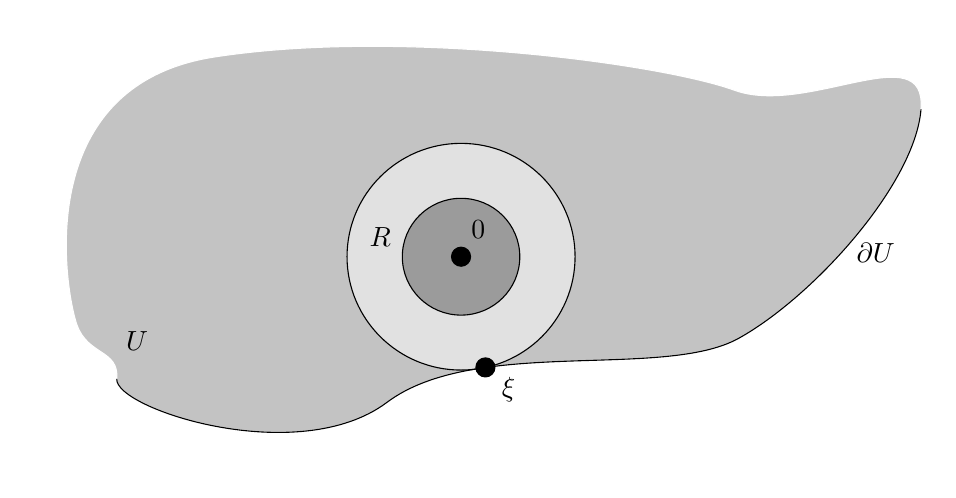
\begin{tikzpicture}[x=0.8pt,y=0.8pt,yscale=-1,xscale=1]
			%uncomment if require: \path (0,300); %set diagram left start at 0, and has height of 300
			
			%Shape: Polygon Curved [id:ds20637273862932082] 
			\draw  [color={rgb, 255:red, 255; green, 255; blue, 255 }  ,draw opacity=1 ][fill={rgb, 255:red, 155; green, 155; blue, 155 }  ,fill opacity=0.6 ] (132,214) .. controls (131,227.4) and (214,254.6) .. (254,224.6) .. controls (294,194.6) and (379,214.6) .. (413,195.6) .. controls (447,176.6) and (492.48,125.93) .. (495.24,92.27) .. controls (498,58.6) and (444,95.6) .. (411,83.6) .. controls (378,71.6) and (260,55.6) .. (176,68.6) .. controls (92,81.6) and (109,175.6) .. (114,189.6) .. controls (119,203.6) and (133,200.6) .. (132,214) -- cycle ;
			%Shape: Ellipse [id:dp8510547001841648] 
			\begin{scope}
				\tikzset{
					render blur shadow/.prefix code={
						\colorlet{black}{rgb, 255:red, 255; green, 255; blue, 255 }  
					}
				}
				
				\draw  [fill={rgb, 255:red, 255; green, 255; blue, 255 }  ,fill opacity=0.5 ] (236,158.8) .. controls (236,130.52) and (259.06,107.6) .. (287.5,107.6) .. controls (315.94,107.6) and (339,130.52) .. (339,158.8) .. controls (339,187.08) and (315.94,210) .. (287.5,210) .. controls (259.06,210) and (236,187.08) .. (236,158.8) -- cycle ;
			\end{scope}
			%Shape: Ellipse [id:dp2967342374206603] 
			\draw  [fill={rgb, 255:red, 155; green, 155; blue, 155 }  ,fill opacity=1 ] (260.97,158.8) .. controls (260.97,144.23) and (272.85,132.42) .. (287.5,132.42) .. controls (302.15,132.42) and (314.03,144.23) .. (314.03,158.8) .. controls (314.03,173.37) and (302.15,185.18) .. (287.5,185.18) .. controls (272.85,185.18) and (260.97,173.37) .. (260.97,158.8) -- cycle ;
			
			%Shape: Circle [id:dp46699756212502197] 
			\draw  [fill={rgb, 255:red, 0; green, 0; blue, 0 }  ,fill opacity=1 ] (283.2,158.8) .. controls (283.2,156.43) and (285.13,154.5) .. (287.5,154.5) .. controls (289.87,154.5) and (291.8,156.43) .. (291.8,158.8) .. controls (291.8,161.17) and (289.87,163.1) .. (287.5,163.1) .. controls (285.13,163.1) and (283.2,161.17) .. (283.2,158.8) -- cycle ;
			%Shape: Circle [id:dp92244155475394] 
			\draw  [fill={rgb, 255:red, 0; green, 0; blue, 0 }  ,fill opacity=1 ] (294.2,208.8) .. controls (294.2,206.43) and (296.13,204.5) .. (298.5,204.5) .. controls (300.87,204.5) and (302.8,206.43) .. (302.8,208.8) .. controls (302.8,211.17) and (300.87,213.1) .. (298.5,213.1) .. controls (296.13,213.1) and (294.2,211.17) .. (294.2,208.8) -- cycle ;
			%Curve Lines [id:da6201100550341501] 
			\draw    (132,214) .. controls (131,227.4) and (214,254.6) .. (254,224.6) .. controls (294,194.6) and (379,214.6) .. (413,195.6) .. controls (447,176.6) and (492.48,125.93) .. (495.24,92.27) ;
			
			% Text Node
			\draw (291,141.4) node [anchor=north west][inner sep=0.75pt]    {$0$};
			% Text Node
			\draw (304.8,212.2) node [anchor=north west][inner sep=0.75pt]    {$\xi$};
			% Text Node
			\draw (135,191.4) node [anchor=north west][inner sep=0.75pt]    {$U$};
			% Text Node
			\draw (465,151.4) node [anchor=north west][inner sep=0.75pt]    {$\partial U$};
			% Text Node
			\draw (245,144.4) node [anchor=north west][inner sep=0.75pt]    {$R$};
		\end{tikzpicture}
	\end{center}
	Per $\lambda$ abbastanza grande abbiamo, in $R$,
	\[ Lv \le C\left( -\lambda^2 +\lambda + 1\right) \le 0.\]
	
	Mostriamo che esiste $\varepsilon > 0 $ tale che per ogni $x \in \partial \textup{B}(0,\frac{r}{2})$ si abbia
	\[ u(\xi) \ge u(x) +\varepsilon v(x). \]
	Se, per assurdo, per ogni $j \in \N\setminus \left\lbrace 0\right\rbrace $ esistesse $x_j \in \partial \textup{B}(0,\frac{r}{2})$ tale che
	\[ u(\xi) < u(x_j) + \frac{1}{j}v(x_j), \]
	dalla compattezza di $\partial \textup{B}(0,\frac{r}{2})$, esisterebbe $(x_{j_k})$ tale che $x_{j_k} \to \tilde{x}$ in $U$ per qualche $\tilde{x} \in U$. Allora $u(\xi) \le u(\tilde{x})$, assurdo.
	
	Osserviamo poi che per ogni $x \in \partial \textup{B}(0,r)$ si ha
	\[ u(\xi) \ge u(x) +\varepsilon v(x), \]
	quindi in definitiva per ogni $x \in \partial R = \partial \textup{B}(0,\frac{r}{2}) \cup \partial \textup{B}(0,r)$ si ha
	\[  u(\xi) \ge u(x) +\varepsilon v(x). \]
	
	Ora, su $R$
	\[ L\left(  u + \varepsilon v -u(\xi)\right)  = Lu +\varepsilon Lv - Lu(\xi) \le -cu(\xi) \le 0 \]
	e quindi, per il Principio del massimo debole,
	\[ \underset{\overline{R}}{\max} \; \left(  u + \varepsilon v -u(\xi)\right) = \underset{\partial R}{\max} \; \left(  u + \varepsilon v -u(\xi)\right) \le 0 \]
	da cui 
	\[   u + \varepsilon v -u(\xi) \le 0\]
	su $\overline{R}$, e quindi in particolare su $R$. In particolare, essendo $\varepsilon v(\xi) = 0$, 
	\[  u + \varepsilon v  \le u(\xi) + \varepsilon v(\xi), \]
	quindi, procedendo come nell'osservazione iniziale,
	\[ \frac{\partial u}{\partial \nu}(\xi) + \varepsilon \frac{\partial v}{\partial \nu}(\xi) \ge 0 \]
	allora
	\begin{align*}
		\frac{\partial u}{\partial \nu}(\xi) &\ge - \varepsilon \frac{\partial v}{\partial \nu}(\xi) = -\varepsilon Dv(\xi) \cdot \nu(\xi) =-\varepsilon Dv(\xi) \cdot \frac{\xi}{r} = \\
		&= -\varepsilon Dv(\xi) \cdot \frac{\xi}{r} = 2\varepsilon \lambda e^{-\lambda r^2}\frac{\xi \cdot \xi}{r} = 2\lambda \varepsilon re^{-\lambda r^2} > 0 
	\end{align*}
	da cui la tesi.
	\par\noindent
	$(a)$ Si tratta di una semplice variante di $(b)$.
\end{proof}

\begin{teorema}\textbf{\emph{(principio del massimo forte)}}\index[analitico]{principio!del massimo!forte}
	Siano $U$ connesso e $u \in C^2(U)\cap C(\overline{U}) $. Supponiamo $c= 0$ in $U$. Valgono i seguenti fatti:
	\begin{enumerate}[$(a)$]
		\item se $Lu \le 0$ in $U$ e $u$ raggiunge il suo massimo su $\overline{U}$ in un punto interno, allora $u$ è costante in $U$,
		\item se $Lu \ge 0$ in $U$ e $u$ raggiunge il suo minimo su $\overline{U}$ in un punto interno, allora $u$ è costante in $U$.
	\end{enumerate}
\end{teorema}
\begin{proof}\hfill
	\par\noindent
	$(a)$ Denotiamo con 
	\[ M = \underset{\overline{U}}{\textup{max}}\; u \]
	\[ C = \left\lbrace x \in U : u(x) = M\right\rbrace. \]
	Per ipotesi $C \ne \emptyset$. Supponiamo, per assurdo, che $u \ne M$. Allora sia 
	\[ V = \left\lbrace x \in U : u(x)< M\right\rbrace.\]
	Sia $y \in V$ tale che $\textup{dist}(y,C) < \textup{dist}(y,\partial U)$ e chiamiamo $\textup{B}$ la più grande palla aperta di centro $y$ che giace in $V$. 
	
	Esiste $\xi \in C$ tale che $\xi \in \partial \textup{B}$. Chiaramente $V$ soddisfa le ipotesi del Lemma di Hopf, pertanto
	\[ \frac{\partial u}{\partial \nu}(\xi) >0, \]
	ma essendo $\xi$ punto di massimo per $u$, $Du(\xi) = 0$, assurdo.
	\par\noindent
	$(b)$ Si tratta di scambiare $u$ con $-u$ nella $(a)$.
\end{proof}

Di particolare interesse è la disuguaglianza di Harnack. Vediamo dapprima il caso $L = \Delta$.
\begin{proposizione}
	Sia $u$ una funzione armonica. Allora per ogni aperto connesso $V$ tale che $\overline{V} \subseteq U$, esiste $C > 0$, dipendente solo da $V$, tale che 
	\[ \underset{V}{\sup} \; u \le C \underset{V}{\inf} \; u. \]
\end{proposizione}
\begin{proof}
	Sia $r = \frac{1}{4}\textup{dist}(V,\partial U)$. Siano $x,y \in V$ tali che $\abs{x-y}\le r$. Per il Teorema della media\footnote{Si rimanda alla 
		\href{https://www.dmf.unicatt.it/~musesti/EDFM/}{dispensa del corso di Equazioni differenziali della fisica matematica} del professor Alessandro Musesti per i dovuti accertamenti.}, 
	\begin{align*}
		u(x) = \fint_{\textup{B}(x,2r)} ud\mathcal{L}^n &= \frac{1}{\mathcal{L}^n(\textup{B}(0,1))(2r)^n} \int_{\textup{B}(x,2r)}ud\mathcal{L}^n \ge \frac{1}{\mathcal{L}^n(\textup{B}(0,1))(2r)^n} \int_{\textup{B}(y,r)}ud\mathcal{L}^n = \\
		&= \frac{1}{2^n} \frac{1}{\mathcal{L}^n(\textup{B}(0,1))(r)^n} \int_{\textup{B}(y,r)}ud\mathcal{L}^n = \frac{1}{2^n} \fint_{\textup{B}(y,r)} = \frac{1}{2^n} u(y). 
	\end{align*}
	Essendo $V$ connesso e $\overline{V}$ compatto, possiamo ricoprire $\overline{V}$ con una catena finita di palle aperte $\textup{B}_i$, con $i = 1,\dots, N$ ed $N$ dipendente solo da $V$, di raggio $r$ con intersezione non vuota e quindi per ogni $x,y \in V$
	\[ u(x) \ge \frac{1}{2^{nN}} u(y). \]
	In altre parole, esiste $C >0$, dipendente solo da $V$, tale che
	\[ \underset{V}{\textup{sup}}\; u \le Cu(x) \]
	e quindi 
	\[ \underset{V}{\textup{sup}}\; u \le C  \underset{V}{\textup{inf}}\; u.\qedhere\]
\end{proof}
Veniamo quindi al caso generale.
\begin{teorema}\textbf{\emph{(disuguaglianza di Harnack)}}\index[analitico]{disuguaglianza!di Harnack}
	Sia $u \in C^2(U)$ una soluzione di 
	\[ Lu = 0 \qquad \textup{in } U \]
	tale che $u\ge 0$ in $U$. Allora per ogni aperto connesso $V$ tale che $\overline{V} \subseteq U$, esiste $C > 0$, dipendente solo da $V,U$ ed $L$, tale che 
	\[ \underset{V}{\sup} \; u \le C \underset{V}{\inf} \; u. \]
\end{teorema}
\begin{proof}
	Limitiamo la dimostrazione al caso $a_{ij} \in C^\infty(U), b = 0, c=0$, ossia
	\[ \sum_{i,j=1}^{n}a_{ij}D^2_{i,j}u = 0 \qquad \textup{in } U. \]
	In particolare, allora $u \in C^\infty(U)$.
	
	Supponiamo inizialmente che $u > 0$ in $U$. Allora possiamo porre
	\[ v = \ln u. \]
	Pertanto, abbiamo che $u = e^v$ e per ogni $i,j = 1,\dots, n$
	\begin{align*}
		D_j u &= e^v D_j v & D^2_{ij}u &= e^v\left( D_i v D_j v + D^2_{i,j}v\right), 
	\end{align*}
	quindi, 
	\[ \sum_{i,j=1}^{n} a_{ij}D^2_{i,j}u = e^v \sum_{i,j=1}^n a_{ij}\left( D_ivD_jv + D^2_{ij}v\right)  = 0 \]
	ossia
	\[ \sum_{i,j=1}^{n}a_{ij}\left( D_ivD_jv + D^2_{i,j}v\right)  = 0 . \]
	In altre parole,
	\[ -\sum_{i,j=1}^{n}a_{ij}D^2_{i,j}v = \sum_{i,j=1}^{n}a_{ij}D_ivD_jv \]
	che, posto 
	\[ w =  \sum_{i,j=1}^{n}a_{ij}D_ivD_jv,\]
	diventa 
	\begin{equation}\label{eq1Harnack}
		-\sum_{i,j=1}^{n}a_{ij}D^2_{i,j}v = w.
	\end{equation}
	Ora, per uniforme ellitticità, esiste $\nu>0$ tale che 
	\[ w \ge \nu \abs{Dv}^2 \ge 0, \]
	allora $\abs{Dv}^2 \le \frac{1}{\nu}w$. Sia $V$ un aperto connesso tale che $\overline{V} \subseteq U$. Mostriamo che $w \in L^\infty(V)$. Innanzitutto, per ogni $k=1,\dots,n$,
	\[ D_k w = \sum_{i,j=1}^{n} D_k a_{ij} D_i v D_j v + \sum_{i,j=1}^{n} a_{ij} D^2_{k,i}v D_j v + \sum_{i,j=1}^{n} a_{ij} D_i v D^2_{k,j} v \]
	e dal fatto che $a_{ij} = a_{ji}$,
	\[ D_k w = \sum_{i,j=1}^{n} D_k a_{ij} D_i v D_j v + \sum_{i,j=1}^{n} a_{ij} D^2_{k,i}v D_j v + \sum_{i,j=1}^{n} a_{ji} D_i v D^2_{k,j} v, \]
	ma essendo nel terzo addendo $i,j$ indici muti, possiamo effettuare la permutazione che li scambia ottenendo
	\[ D_k w = \sum_{i,j=1}^{n} D_k a_{ij} D_i v D_j v + 2\sum_{i,j=1}^{n} a_{ij} D^2_{k,i}v D_j v. \]
	In maniera del tutto simile, per ogni $l = 1,\dots, n$,
	\[ D^2_{l,k} w = 2\sum_{i,j=1}^{n} a_{ij} D^3_{l,k,i}v D_j v + 2\sum_{i,j=1}^{n} a_{ij} D^2_{k,i}v D^2_{l,j}v + R_1 \]
	dove 
	\[ R_1 = \sum_{i,j=1}^{n} D^2_{l,k} a_{ij} D_i v D_j v + 2\sum_{i,j=1}^{n} D_k a_{ij} D^2_{l,i} v D_j v + 2\sum_{i,j=1}^{n} D_l a_{ij} D^2_{k,i} v D_j v. \]
	In particolare, esiste $C>0$, dipendente solo dagli $a_{ij}$ e da $V$, tale che
	\[ \abs{R_1} \le C\left( \abs{D^2 v}\abs{Dv} + \abs{Dv}^2\right)  \]
	e, per la disuguaglianza di Young pesata, per ogni $\varepsilon > 0$, 
	\[ \abs{R_1} \le \varepsilon \abs{D^2v}^2 + \frac{C}{\varepsilon}\abs{Dv}^2. \]
	Pertanto, 
	\[ -\sum_{k,l=1}^{n}a_{kl}D^2_{k,l}w = -2 \sum_{i,j=1}^na_{ij}D_j v \left( \sum_{k,l=1}^n a_{kl}D^3_{l,k,i} v\right)  - 2 \sum_{i,j,k,l=1}^{n} a_{ij}a_{kl}D^2_{k,i}v D^2_{l,k} v + R_2 \]
	dove 
	\[ R_2 = -\sum_{k,l=1}^n a_{kl} R_1 \]
	e chiaramente esiste $C>0$, dipendente solo dagli $a_{ij}$ e da $V$, tale che
	\[ \abs{R_2} \le \varepsilon \abs{D^2 v}^2 + \frac{C}{\varepsilon}\abs{Dv}^2. \]
	D'altra parte, per l'equazione \eqref{eq1Harnack},
	\[ D_k w = D_k \left(-\sum_{i,j=1}^{n}a_{ij}D^2_{i,j}v\right) = - \sum_{i,j=1}^na_{ij}D^3_{k,i,j}v - \sum_{i,j=1}^n D_ka_{ij} D^2_{i,j} v.  \]
	Chiamiamo 
	\[ R_3 = - \sum_{i,j=1}^n D_ka_{ij} D^2_{i,j} v, \]
	allora esiste $C>0$, dipendente solo dagli $a_{ij}$ e da $V$, tale che
	\[ \abs{R_3} \le C \abs{D^2v}. \]
	A questo punto, posto
	\[ \bar{b}_k = -2\sum_{l=1}^{n}a_{kl}D_l v, \]
	abbiamo subito che esiste $C>0$, dipendente solo dagli $a_{ij}$ e da $V$, tale che  $\abs{\bar{b}} \le C \abs{Dv}$. Inoltre, risulta che 
	\[ \sum_{k=1}^{n} \bar{b}_k D_k w = -\sum_{i,j,k=1}^{n} a_{ij}\bar{b}_k D^3_{k,i,j} v + R_4 \]
	dove 
	\[ R_4 = -\sum_{k=1}^{n}\bar{b}_k R_3 \]
	e quindi esiste $C>0$, dipendente solo dagli $a_{ij}$ e da $V$, tale che
	\[ \abs{R_4} \le \sum_{k=1}^{n}\abs{\bar{b}_k} \abs{R_3} \le 2C\sum_{k,l=1}^{n} \abs{a_{kl}} \abs{D_l v}\abs{D^2v} \le C\abs{D v} \abs{D^2 v}   \]
	e, per la disuguaglianza di Young pesata, per ogni $\varepsilon > 0$
	\[ \abs{R_4} \le \varepsilon \abs{D^2 v}^2 + \frac{C}{\varepsilon}\abs{Dv}^2. \]
	Osserviamo invece che 
	\[ \sum_{i,j,k=1}^{n} a_{ij}\bar{b}_k D^3_{k,i,j} v = 2 \sum_{i,j=1}^n a_{ij}\left( \sum_{k,l=1}^n a_{kl} D_l v D^3_{k,i,j} v\right)  \]
	ed effettuando la permutazione di indici che scambia $k,i$ e $l,j$ si ottiene
	\[  \sum_{i,j,k=1}^{n} a_{ij}\bar{b}_k D^3_{k,i,j} v = 2 \sum_{i,j=1}^na_{ij}D_j v \left( \sum_{k,l=1}^n a_{kl}D^3_{l,k,i} v\right). \]
	Alla luce di ciò, 
	\[ -\sum_{k,l=1}^{n}a_{kl}D^2_{k,l}w + \sum_{k=1}^{n} \bar{b}_k D_k w =  - 2 \sum_{i,j,k,l=1}^{n} a_{ij}a_{kl}D^2_{k,i}v D^2_{l,k} v + R_2 + R_4.  \]
	Ora, sempre per uniforme ellitticità, 
	\begin{align*}
		\sum_{i,j,k,l=1}^{n} a_{ij}a_{kl}D^2_{k,i}v D^2_{l,k} v &= \sum_{i,j=1}^{n}  a_{ij} \left( \sum_{k,l=1}^n a_{kl} D^2_{k,i}v D^2_{l,k} v \right) \ge \sum_{i,j=1}^{n}  a_{ij} \left( \nu \abs{D^2 v}^2\right) = \\
		&= \nu \abs{D^2 v}^2 \sum_{i,j=1}^{n}  a_{ij} \ge   \nu \abs{D^2 v}^2  \nu = \nu^2 \abs{D^2 v}^2,
	\end{align*}
	quindi scelto $\varepsilon = \frac{\nu^2}{4}$, esiste $C>0$, dipendente solo dagli $a_{ij}$ e da $V$, tale che
	\[ -\sum_{k,l=1}^{n}a_{kl}D^2_{k,l}w + \sum_{k=1}^{n} \bar{b}_k D_k w  \le -\frac{\nu^2}{2}\abs{D^2 v}^2 + C\abs{Dv}^2. \]
	Sia $W$ un aperto tale che $\overline{V} \subseteq W \subseteq \overline{W} \subseteq U$. Consideriamo la funzione di cut-off $\zeta \in C^\infty_c(U)$ tale che $0\le \zeta \le 1, \zeta = 1$ su $V$, $\zeta = 0$ su $\R^n \setminus W$. Consideriamo $z = \zeta ^4 w \in C_c(U)$.\footnote{In realtà è più regolare di così.} Allora,
	\[ D_k z = 4 \zeta^3 D_k \zeta w + \zeta^4 D_k w \]
	e 
	\[ D^2_{l,k} z = 12\zeta^2 D_l \zeta D_k \zeta w + 4 \zeta^3 D^2_{l,k} \zeta w + 4\zeta^3 D_k\zeta D_lw + 4\zeta^3D_l\zeta D_kw + \zeta^4 D^2_{l,k}w. \]
	Inoltre, esisterà un qualche $\xi \in U$ tale che $z$ ammette massimo su $U$ in $\xi$. In particolare, essendo $w \ge 0$, $\zeta(\xi)> 0$ e $Dz(\xi) = 0$, ossia
	\[ 4\zeta^3(\xi)D_k\zeta(\xi) w(\xi) + \zeta^4(\xi)D_kw(\xi)  =0 \]
	e dividendo per $\zeta^3(\xi)$
	\begin{equation}\label{eq2Harnack}
		4D_k\zeta(\xi) w(\xi) + \zeta(\xi)D_kw(\xi)  =0.
	\end{equation}
	Ora, 
	\begin{align*}
		-\sum_{k,l=1}^n a_{kl}D^2_{k,l}z = &-\sum_{k,l=1}^n a_{kl} \zeta^4 D^2_{l,k}w + \\
		& -\sum_{k,l=1}^n a_{kl}\left(12\zeta^2 D_l \zeta D_k \zeta w + 4 \zeta^3 D^2_{l,k} \zeta w + 4\zeta^3 D_k\zeta D_lw + 4\zeta^3D_l\zeta D_kw\right)
	\end{align*}
	mentre
	\[ \sum_{k=1}^n \bar{b}_k D_k z =  \sum_{k=1}^n \bar{b}_k \zeta^4 D_k w + \sum_{k=1}^n \bar{b}_k 4 \zeta^3 D_k \zeta w. \]
	Posto
	\begin{align*}
		R_5 =  &-\sum_{k,l=1}^n a_{kl}\left(12\zeta^2 D_l \zeta D_\zeta z w + 4 \zeta^3 D^2_{l,k} \zeta w + 4\zeta^3 D_k\zeta D_lw + 4\zeta^3D_l\zeta D_kw\right) + \\
		&+ \sum_{k=1}^n \bar{b}_k 4 \zeta^3 D_k \zeta w,
	\end{align*}
	esiste $C>0$, dipendente solo da $U,V$ ed $L$, tale che
	\[ \abs{R_5} \le C\left( \zeta^2 \abs{w} + \zeta^3 \abs{w} + \zeta^3\abs{Dw} + \abs{\bar{b}} \zeta^3 \abs{w} \right) \le C\left( \zeta^2 \abs{w} + \zeta^3\abs{Dw} + \zeta^3\abs{Dv}  \abs{w} \right).  \]
	Essendo quindi $\xi$ un punto di massimo, e siccome il prodotto scalare tra una matrice definita positiva ed una semidefinita negativa è negativo,
	\begin{align*}
		0\le  -\sum_{k,l=1}^n a_{kl}(\xi)D^2_{k,l}z(\xi) + \sum_{k=1}^n \bar{b}_k(\xi) D_k z(\xi) = &\zeta^4(\xi)\left(-\sum_{k,l=1}^n a_{kl}(\xi) D^2_{l,k}w(\xi) + \right. \\
		& +\left.\sum_{k=1}^n \bar{b}_k(\xi) D_k w(\xi)\right) +R_5(\xi),
	\end{align*}
	ma, per l'equazione \eqref{eq2Harnack}, $\abs{Dw(\xi)} \le C \abs{w(\xi)}$ e quindi 
	\[ \abs{R_5(\xi)} \le C \left( \zeta^2(\xi)\abs{w(\xi)} + \zeta^3(\xi)\abs{Dv(\xi)}\abs{w(\xi)}\right). \]
	Allora,
	\begin{align*}
		0 &\le \zeta^4(\xi)\left(-\sum_{k,l=1}^n a_{kl}(\xi) D^2_{l,k}w(\xi) +\sum_{k=1}^n \bar{b}_k(\xi) D_k w(\xi)\right) +R_5(\xi) \le \\
		&\le \zeta^4(\xi)\left( -\frac{\nu^2}{2}\abs{D^2 v(\xi)}^2 + C\abs{Dv(\xi)}^2\right) + C \left( \zeta^2(\xi)\abs{w(\xi)} + \zeta^3(\xi)\abs{Dv(\xi)}\abs{w(\xi)}\right)
	\end{align*}
	da cui, ricordando che $\abs{Dv}^2 \le \abs{w}$ e osservando che, per \eqref{eq1Harnack}, $\abs{w}\le \abs{D^2v}$ ,
	\begin{align*}
		\frac{\nu^2}{2}\zeta^4(\xi) \abs{D^2v(\xi)}^2 &\le C\zeta^4(\xi) \abs{Dv(\xi)}^2 + C\zeta^2(\xi)\abs{w(\xi)}+\zeta^3(\xi)\abs{Dv(\xi)}\abs{w(\xi)} \le \\
		&\le C\zeta^4(\xi) \abs{w(\xi)} + C\zeta^2(\xi)\abs{w(\xi)}+\zeta^3(\xi)\abs{Dv(\xi)}\abs{D^2v(\xi)}.
	\end{align*}
	Ora, per la disuguaglianza di Young pesata con $\varepsilon = \frac{\nu^2}{4}\zeta(\xi)$,
	\begin{align*}
		\zeta^3(\xi)\abs{Dv(\xi)}\abs{D^2v(\xi)} &\le \frac{\nu^2}{4}\zeta^4(\xi) \abs{D^2v(\xi)}^2 + C\zeta^3(\xi)\abs{Dv(\xi)}^2 \le \\
		&\le \frac{\nu^2}{4}\zeta^4(\xi) \abs{D^2v(\xi)}^2 + C\zeta^3(\xi)\abs{w(\xi)},
	\end{align*}
	quindi
	\[ \frac{\nu^2}{4}\zeta^4(\xi) \abs{D^2v(\xi)}^2 \le C\zeta^2(\xi)\abs{w(\xi)} \le C\abs{w(\xi)}. \]
	Allora, essendo $\abs{w(\xi)}^2\le C\abs{D^2v}^2$,
	\[ \zeta^4(\xi)\abs{w(\xi)}^2 \le C\abs{w(\xi)}. \]
	In definitiva, 
	\[ \underset{V}{\max} \; z \le C\]
	ed essendo $\zeta = 1$ su $V$ possiamo concludere che $\norm{w}_{L^\infty(V)} < +\infty$, ossia $w \in L^\infty(V)$. 
	
	Allora, anche $Dv \in L^\infty(V)$. A questo punto, dati $x,y \in V$, per la disuguaglianza di Lagrange\footnote{Qui si usa la connessione.}, esiste $\eta$ nel segmento congiungente $x,y$ tale che
	\[ \frac{u(x)}{u(y)} = e^{v(x)-v(y)} \le e^{\abs{x-y}\abs{Dv(\xi)}} \le e^{\textup{diam}(V)\norm{Dv}_{L^\infty(V)}} < +\infty.  \]
	Possiamo quindi affermare che per ogni $x,y \in V$
	\[ u(x) \le C u(y) \]
	ossia 
	\[ \underset{V}{\textup{sup}}\; u \le Cu(y) \]
	e quindi 
	\[ \underset{V}{\textup{sup}}\; u \le C  \underset{V}{\textup{inf}}\; u.\]
	
	Per quanto riguarda il caso generale, sia $\varepsilon >0 $ tale che 
	\[ \tilde{u} = u + \varepsilon >0. \]
	Applicando il caso precedente a $\tilde{u}$ e poi passando al limite per $\varepsilon \to 0$ si ha la tesi.
\end{proof}
\begin{osservazione}
	La disuguaglianza di Harnack mostra che i valori di soluzioni non negative di problemi ellittici, in una regione lontana dal bordo, sono comparabili: per ogni $x,y \in V$ tale che $\overline{V} \subseteq U$, 
	\[ \frac{1}{C} u(y) \le u(x) \le Cu(y). \]
	In particolare, se esiste $x \in V$ tale che $u(x) >0$, allora $u> 0$ in $V$.
\end{osservazione}
\section{Problemi agli autovalori}
I risultati di questa sezione sono gli analoghi nel caso di problemi ellittici di alcune affermazioni classiche di Algebra Lineare riguardo matrici simmetriche reali.

Nel corso di questa sezione consideriamo operatori in forma di divergenza del tipo 
\[ Lu = -\sum_{i,j=1}^{n}D_{j}(a_{ij}D_iu)\]
con $a_{ij} \in C^\infty(\overline{U})$. Oltre alle usuali ipotesi di struttura, considereremo anche $U$ connesso.
\begin{teorema}
	Valgono i seguenti fatti:
	\begin{enumerate}[$(a)$]
		\item ogni autovalore di $L$ è reale,
		\item contando ogni autovalore con la relativa molteplicità (finita), 
		\[ \Sigma = \left\lbrace \lambda_k : k \in \N\setminus\left\lbrace 0\right\rbrace \right\rbrace  \]
		dove 
		\[ 0 < \lambda_1 \le \lambda_2 \le \dots \]
		e $\lambda_k \to +\infty$ se $k \to +\infty$,
		\item esiste una base hilbertiana $(w_k)$ di $L^2(U)$ costituita da autovettori $w_{k} \in H^1_0(U)$ relativi agli autovalori $\lambda_k$, ossia per ogni $k \in \N\setminus\left\lbrace 0\right\rbrace$
		\[ \begin{cases}
			Lw_k = \lambda_k w_k & \textup{in } U,\\
			w_k = 0 & \textup{su } \partial U.
		\end{cases} \]
	\end{enumerate}
\end{teorema}
\begin{proof}
	In modo analogo quanto visto nei Teoremi di esistenza, si dimostra che
	\[ S = L^{-1} : L^2(U) \to L^2(U)\]
	è un operatore compatto.
	
	Mostriamo che $S$ è simmetrico. Siano $f,g \in L^2(U)$. Allora esistono e sono uniche $u,v \in H^1_0(U)$ soluzioni deboli, rispettivamente, di 
	\begin{align*}
		&\begin{cases}
			Lu = f & \textup{in } U,\\
			u = 0 & \textup{su } \partial U,
		\end{cases} & &\begin{cases}
			Lu = g & \textup{in } U,\\
			u = 0 & \textup{su } \partial U,
		\end{cases} 
	\end{align*}
	ossia $Sf = u$ e $Sg = v$. Per la formulazione debole, 
	\[ (Sf|g)_2 = (u|g)_2 = B(v,u) \]
	\[ (f|Sg)_2 = (f|v)_2 = B(u,v) \]
	e per simmetria di $B$, si ha $(Sf|g)_2 =(f|Sg)_2$, da cui $S$ è simmetrico. Inoltre, per ogni $f \in L^2(U)$
	\[ (Sf|f)_2 = (u|f)_2 = B(u,u) \ge 0. \]
	Dal Teorema Spettrale per operatori compatti, segue dunque che gli autovalori di $S$ sono tutti reali, strettamente positivi e le corrispondenti autofunzioni formano una base hilbertiana di $L^2(U)$. 
	
	Dal fatto che per $\eta \ne 0$, si ha che 
	\[ Sw = \eta w \Longleftrightarrow Lw = \lambda w \]
	con $\lambda = \frac{1}{\eta}$, segue la tesi.
\end{proof}
\begin{definizione}
	Chiamiamo $\lambda_1$ \emph{autovalore principale}\index[analitico]{autovalore!principale} o \emph{primo autovalore} di $L$.
\end{definizione}

\begin{lemma}
	Sia $H$ uno spazio di Hilbert ed $M \subseteq H$ non vuoto. Allora $\overline{\textup{span}(M)} = H$ se e solo se $M^\perp = \left\lbrace 0\right\rbrace $.
\end{lemma}
\begin{proof}
	Omettiamo la dimostrazione.
\end{proof}

\begin{teorema}\textbf{\emph{(principio variazionale per l'autovalore principale)}}\index[analitico]{principio! variazionale! per l'autovalore principale}
	Valgono i seguenti fatti:
	\begin{enumerate}[$(a)$]
		\item si ha che
		\[ \lambda_1 = \min \Set{B(u,u): u \in H^1_0(U), \norm{u}_{L^2(U)}=1}, \]
		\item il minimo è raggiunto in $w_1>0$ tale che 
		\[ \begin{cases}
			Lw_1 = \lambda_1 w_1 & \textup{in } U,\\
			w_1 = 0 & \textup{su } \partial U,
		\end{cases} \]
		\item se $u \in H^1_0(U)$ è una soluzione debole di 
		\[ \begin{cases}
			Lu = \lambda_1 u & \textup{in } U,\\
			u = 0 & \textup{su } \partial U,
		\end{cases} \]
		allora esiste $k \in \R$ tale che $u = k w_1$.
	\end{enumerate}
\end{teorema}
\begin{proof}
	Per la $(c)$ del Teorema precedente e la formulazione variazionale, per ogni $k,l \in \N\setminus\left\lbrace 0\right\rbrace $, 
	\[ B(w_k,w_l) = \lambda_k \delta_k^l \]
	e quindi 
	\[ B\left( \frac{w_k}{\sqrt{\lambda_k}},\frac{w_l}{\sqrt{\lambda_l}}\right)  =\delta_k^l. \]
	Inoltre, se $u \in H^1_0(U)$ e $\norm{u}_{L^2(U)}=1$, posto $d_k = (u|w_k)_{L^2(U)}$, si ha
	\begin{equation}\label{serie1primoautovalore}
		u = \sum_{k=1}^{\infty}d_k w_k\footnote{La serie converge in $L^2(U)$.}
	\end{equation}
	e, per la disuguaglianza di Bessel--Parseval,
	\[ \sum_{k=1}^{\infty} d_k^2 = \norm{u}_{L^2(U)}=1. \]
	
	Consideriamo $H^1_0(U)$ munito del prodotto scalare $B(\;,\;)$. Mostriamo che la norma indotta $\norm{\;}_B$ è equivalente alla norma $\norm{\;}_{H^1_0(U)}$. Innanzitutto, per ogni $u \in H^1_0(U)$, per uniforme ellitticità
	\[ \norm{u}_B^2 = \sum_{i,j=1}^n \int_{U} a_{ij}D_iuD_ju d\mathcal{L}^n \ge \nu \int_{U} \abs{Du}^2d\mathcal{L}^n = \nu \norm{u}^2_{H^1_0(U)}. \]
	Viceversa, 
	\[ \norm{u}^2_{B} \le C \int_{U} \abs{Du}^2d\mathcal{L}^n = C\norm{u}^2_{H^1_0(U)}. \]
	In definitiva, anche $\left( H^1_0(U),\norm{\;}_B\right)  $ è uno spazio di Hilbert su $\R$.
	
	Per quanto osservato inizialmente, $\left( \frac{w_k}{\sqrt{\lambda_k}}\right) $ è un sottoinsieme ortonormale di $H^1_0(U)$. Mostriamo che è una base hilbertiana di $H^1_0(U)$ con il prodotto scalare sopra introdotto. Questo fatto è equivalente ad affermare che 
	\[ \forall\; u \in H^1_0(U): \bigl( B(w_k,u) = 0 \textup{ per ogni } k \in \N\setminus \left\lbrace 0\right\rbrace \bigr) \Longrightarrow u = 0.\footnote{Sia $u \in H^1_0(U)$ tale che per ogni $k \in \N\setminus \left\lbrace 0\right\rbrace$, $B(w_k,u) = 0$. Se $\left( \frac{w_k}{\sqrt{\lambda_k}}\right) $ è una base hilbertiana,
		\begin{align*}
			u &= \sum_{k=1}^\infty l_k \frac{w_k}{\sqrt{\lambda_k}} & l_k &=  B\left( u,\frac{w_k}{\sqrt{\lambda_k}}\right) =\frac{1}{\sqrt{\lambda_k}} B(w_k,u)= 0,
		\end{align*}
		allora $u= 0$. Viceversa, sia $M = \left\lbrace \frac{w_k}{\sqrt{\lambda_k}} : k \in \N\setminus \left\lbrace 0\right\rbrace\right\rbrace  .$ Per ipotesi, $M^\perp = \left\lbrace 0\right\rbrace $, allora per il Lemma precedente si ha $\overline{\textup{span}(M)} = H^1_0(U)$. Se $u \in H^1_0(U)$, allora esiste $(u_h)$ in $\textup{span}(M)$ tale che $u_h \to u$ in $H^1_0(U)$. Deve essere 
		\[ u_h = \sum_{k=1}^{\infty} a_k^{(h)}\frac{w_k}{\sqrt{\lambda_k}} \]
		dove solo un numero finito di $\alpha_k^{(h)}$ è non nullo. Siccome $B\left( u_h,\frac{w_l}{\sqrt{\lambda_l}}\right)  = \alpha_l^{(h)}$, sfruttando la continuità del prodotto scalare, $B\left( u,\frac{w_l}{\sqrt{\lambda_l}}\right)  = B\left( \lim\limits_{h} u_h,\frac{w_l}{\sqrt{\lambda_l}}\right)  =  \lim\limits_{h} \alpha_l^{(h)}$ e per il Teorema della convergenza dominata (versione discreta), si ha $u = \lim\limits_{h} u_h = \sum\limits_{k=1}^{\infty} B\left( u,\frac{w_k}{\sqrt{\lambda_k}}\right) \frac{w_k}{\sqrt{\lambda_k}}$.} \]
	Ma quest'ultima affermazione è vera in quanto, essendo $(w_k)$ una base hilbertiana di $L^2(U)$, allora se per ogni $k \in \N\setminus \left\lbrace 0\right\rbrace$, 
	\[ B(w_k,u) = \lambda_k (w_k | u)_{L^2(U)} = 0 \]
	allora $u = 0$. 
	
	Di conseguenza, 
	\[ u = \sum_{k=1}^{\infty} \mu_k \frac{w_k}{\sqrt{\lambda_k}}\footnote{La serie converge in $H^1_0(U)$.} \]
	dove $\mu_k = B\left( u,\frac{w_k}{\sqrt{\lambda_k}}\right) $.
	
	Ora, siccome $\mu_k = d_k \sqrt{\lambda_k}$, la serie \eqref{serie1primoautovalore} converge anche in $H^1_0(U)$. Allora, sfruttando la continuità del prodotto scalare,
	\[ B(u,u) = B\left( \sum_{k=1}^{\infty} d_k w_k , \sum_{i=1}^{\infty} d_i w_i\right)  = \lim\limits_{m} \sum_{k,i=1}^{m} d_kd_iB(w_k,w_i) = \lim\limits_{m} \sum_{k=1}^{m} d_k^2\lambda_k \ge \lambda_1 \sum_{k=1}^{\infty} d_k^2 = \lambda_1. \]
	Siccome $B(w_1,w_1) = \lambda_1$, allora $w_1$ realizza il precedente minimo. 
	
	Mostriamo che se $u \in H^1_0(U)$ e $\norm{u}_{L^2(U)}=1$, $u$ è soluzione debole di 
	\[ \begin{cases}
		Lu = \lambda_1 u & \textup{in } U,\\
		u = 0 & \textup{su } \partial U,
	\end{cases} \]
	se e solo se $B(u,u) = \lambda_1$. Se $u$ è soluzione debole del problema precedente, per ogni $v \in H^1_0(U)$, $B(u,v) = \lambda_1 (u|v)_{L^2(U)}$. Scelto $v= u$, si ha $B(u,u) = \lambda_1 \norm{u}^2_{L^2(U)} = \lambda_1$. Viceversa,
	\[ \sum_{k=1}^\infty d^2_k \lambda_1 = \lambda_1 = B(u,u) = \sum_{k=1}^{\infty} d_k^2 \lambda_k \]
	allora
	\[ \sum_{k=1}^{\infty} (\lambda_k - \lambda_1) d_k^2 = 0 \]
	e di conseguenza deve essere $d_k = 0$ se $\lambda_k > \lambda_1$. Siccome $\lambda_1$ ha molteplicità finita, 
	\[ u = \sum_{k=1}^{m} (u|w_k)_{L^2(U)} w_k \]
	per qualche $m$, dove i $w_k$ sono autovettori relativi all'autovalore $\lambda_1$. Allora
	\[ Lu = \sum_{k=1}^{m} (u|w_k)_{L^2(U)} Lw_k = \lambda_1 u. \] 
	
	Mostriamo che se $u \in H^1_0(U)$ è una soluzione debole del problema precedentemente introdotto allora $u = 0$ oppure ha segno definito\footnote{Si intende che è strettamente positiva oppure strettamente negativa in $U$.}. Per fare ciò, supponiamo $u$ non nulla, allora senza perdita di generalità possiamo prenderla tale che $\norm{u}_{L^2(U)} = 1$. Posto,
	\begin{align*}
		\alpha &= \int_{U} (u^+)^2 d\mathcal{L}^n, & \beta &= \int_{U} (u^-)^2 d\mathcal{L}^n
	\end{align*}
	allora $\alpha + \beta = 1$. Osserviamo che $u^{\pm} \in H^1_0(U)$ con 
	\begin{align*}
		Du^+ &= \begin{cases}
			Du & \textup{q.o. su } \left\lbrace u \ge 0 \right\rbrace ,\\
			0 & \textup{q.o. su } \left\lbrace u \le 0 \right\rbrace ,
		\end{cases}
		&
		Du^- &= \begin{cases}
			0 & \textup{q.o. su } \left\lbrace u \ge 0 \right\rbrace ,\\
			-Du & \textup{q.o. su } \left\lbrace u \le 0 \right\rbrace.
		\end{cases}
	\end{align*}
	e 
	\begin{align*}
		B(u^+,u^-) &= \sum_{i,j=1}^n \int_U a_{ij} D_i u^+ D_j u^- d\mathcal{L}^n = \\
		& =\sum_{i,j=1}^n \int_{U \cap \left\lbrace u \ge 0 \right\rbrace} a_{ij} D_i u^+ D_j u^- d\mathcal{L}^n + \sum_{i,j=1}^n \int_{U \cap \left\lbrace u \le 0 \right\rbrace} a_{ij} D_i u^+ D_j u^- d\mathcal{L}^n = 0.
	\end{align*}
	Ora,
	\begin{align*}
		\lambda_1 &= B(u,u) = B(u^+,u^+) + B(u^-,u^-) + 2B(u^+,u^-) \ge \\
		&\ge \lambda_1 \norm{u^+}^2_{L^2(U)} + \lambda_1\norm{u^-}_{L^2(U)} = (\alpha + \beta) \lambda_1 = \lambda_1,
	\end{align*}
	allora deve essere
	\begin{align*}
		B(u^+,u^+) &= \lambda_1 \norm{u^+}^{2}_{L^2(U)}, & B(u^-,u^-) &= \lambda_1 \norm{u^-}^{2}_{L^2(U)}.
	\end{align*}
	Per il passaggio precedente quindi $u^+$ e $u^-$ sono soluzioni deboli dei problemi
	\begin{align*}
		&\begin{cases}
			Lu^+ = \lambda_1 u^+ & \textup{in } U,\\
			u^+ = 0 & \textup{su } \partial U,
		\end{cases} & &\begin{cases}
			Lu^- = \lambda_1 u^- & \textup{in } U,\\
			u^- = 0 & \textup{su } \partial U.
		\end{cases}
	\end{align*} 
	Ma essendo gli $a_{ij} \in C^\infty(U)$, $u^+ \in C^\infty(U)$ e 
	\[ Lu^+ = \lambda_1 u^+ \ge 0 \textup{ in } U. \]
	In definitiva, $u^+$ è una supersoluzione. Per il Principio del massimo forte quindi $u^+ >0$ in $U$ oppure $u^+ = 0$ in $U$. Un argomento analogo vale per $u^-$.
	
	Sia ora $u$ una soluzione debole non nulla del problema introdotto. Per quanto visto sopra, 
	\[ \int_U w_1 d\mathcal{L}^n \ne 0 \]
	e quindi esiste $k \in \R$ tale che 
	\[ \int_U \left( u-kw_1\right) d\mathcal{L}^n = 0. \]
	Ma 
	\[ L\left( u-kw_1\right)  = Lu -kLw_1 = \lambda_1 u - k Lw_1 = \lambda_1 \left( u-kw_1\right)  \]
	quindi anche $u-kw_1$ è soluzione del problema. Ma allora deve essere $u = kw_1$ in $U$.
\end{proof}
\begin{osservazione}
	L'affermazione $(c)$ del Principio variazionale per l'autovalore principale corrisponde a dire che $\lambda_1$ è \emph{semplice}. In particolare,
	\[ 0<\lambda_1 < \lambda_2 \le \lambda_3 \le \dots \]
\end{osservazione}
\begin{osservazione}
	L'affermazione $(a)$ del Principio variazionale per l'autovalore principale è una caratterizzazione di $\lambda_1$ attraverso un problema di minimo vincolato ed è nota come \emph{formula di Rayleigh}. Si può dimostrare, grazie all'omogeneità di $B(u,u)$, che è equivalente al problema di minimo libero
	\[ \lambda_1 = \underset{\underset{u \ne 0}{u \in H^1_0(U)}}{\min}\; \frac{B(u,u)}{\norm{u}_{L^2(U)}^2}. \] 
	Osserviamo infatti che 
	\[ \frac{B(u,u)}{\norm{u}_{L^2(U)}^2} = B\left( \frac{u}{\norm{u}_{L^2(U)}},\frac{u}{\norm{u}_{L^2(U)}}\right) \]
	e  
	\[ \norm*{\frac{u}{\norm{u}_{L^2(U)}}}_{L^2(U)}=1, \]
	allora
	\[ \lambda_1 \le \frac{B(u,u)}{\norm{u}_{L^2(U)}^2} \]
	e quindi 
	\[ \lambda_1 \le \underset{\underset{u \ne 0}{u \in H^1_0(U)}}{\min}\; \frac{B(u,u)}{\norm{u}_{L^2(U)}^2}. \]
	Viceversa, se $u \in H^1_0(U)$ e $\norm{u}_{L^2(U)} = 1$, allora
	\[ B(u,u) = \frac{B(u,u)}{\norm{u}^2_{L^2(U)}} \ge \underset{\underset{u \ne 0}{u \in H^1_0(U)}}{\min}\; \frac{B(u,u)}{\norm{u}_{L^2(U)}^2} \]
	da cui 
	\[ \lambda_1 \ge \underset{\underset{u \ne 0}{u \in H^1_0(U)}}{\min}\; \frac{B(u,u)}{\norm{u}_{L^2(U)}^2}.\]
\end{osservazione}

\begin{teorema}
	Siano $X$ uno spazio di Hilbert su $\K$ separabile e $S: X \to X$ un operatore lineare compatto e autoaggiunto. Allora esiste una base hilbertiana di $X$ composta da autovettori di $S$.
\end{teorema}
\begin{proof}
	Omettiamo la dimostrazione.
\end{proof}

Consideriamo l'operatore $S: L^2(U) \to L^2(U)$ tale che 
\[ Sf= u, \]
dove $u \in H^1_0(U)$ è l'unica soluzione debole del problema di Dirichlet
\[ \begin{cases}
	-\Delta u = f & \textup{in } U, \\
	u = 0 & \textup{su } \partial U.
\end{cases} \footnote{In altre parole $S$ è l'operatore inverso di $-\Delta$ (debole).}\]
In particolare, $\textup{Im}(S) \subseteq H^1_0(U)$. Chiaramente $S$ è lineare e per ogni $f,g \in L^2(U)$, dette $u = Sf$ e $v = Sg$,
\[ (Sf|g)_{L^2(U)} = (u|g)_{L^2(U)} = \int_U Du \cdot Dv d\mathcal{L}^n = (f|v)_{L^2(U)} = (f|Sg)_{L^2(U)},\]
quindi è pure autoaggiunto. Sia ora $(f_j)$ in $L^2(U)$ limitata. Dette $u_j = Sf_j \in H^1_0(U)$, dalla formulazione variazionale combinata con la disuguaglianza di Holder e la disuguaglianza di Poincaré,
\[ \norm{u_j}^2_{H^1_0(U)} = \int_U \abs{Du_j}^2 d\mathcal{L}^n = \int_U f_j u_j d\mathcal{L}^n \le \norm{f_j}_{L^2(U)} \norm{u_j}_{L^2(U)} \le C\norm{f_j}_{L^2(U)}\norm{u_j}_{H^1_0(U)},\]
quindi $(u_j)$ limitata in $H^1_0(U)$. Per il Teorema di Rellich--Kondrachov, esistono $(u_{j_k})$ e $u \in H^1_0(U)$ tale che $u_{j_k} \to u$ in $L^2(U)$. In particolare, $S$ è compatto. Allora, per il Teorema precedente, esiste $(w_k)$ base hilbertiana di $L^2(U)$ tale che 
\[ Sw_k = \lambda_k w_k. \]
In particolare, $(w_k)$ in $H^1_0(U)$ e
\[ -\Delta w_k = \frac{1}{\lambda_k} w_k \]
in senso debole, quindi
\[ \int_U Dw_h \cdot Dw_k d\mathcal{L}^n = \frac{1}{\lambda_k}  (w_h|w_k)_{L^2(U)},\]
segue che $(w_k)$ è una base hilbertiana di $H^1_0(U)$ costituita da autovettori di $-\Delta$. In particolare, da quanto visto sulla teoria della regolarità, le $w_k$ sono lisce.